\documentclass[12pt,]{book}
\usepackage{lmodern}
\usepackage{amssymb,amsmath}
\usepackage{ifxetex,ifluatex}
\usepackage{fixltx2e} % provides \textsubscript
\ifnum 0\ifxetex 1\fi\ifluatex 1\fi=0 % if pdftex
  \usepackage[T1]{fontenc}
  \usepackage[utf8]{inputenc}
\else % if luatex or xelatex
  \ifxetex
    \usepackage{mathspec}
  \else
    \usepackage{fontspec}
  \fi
  \defaultfontfeatures{Ligatures=TeX,Scale=MatchLowercase}
\fi
% use upquote if available, for straight quotes in verbatim environments
\IfFileExists{upquote.sty}{\usepackage{upquote}}{}
% use microtype if available
\IfFileExists{microtype.sty}{%
\usepackage{microtype}
\UseMicrotypeSet[protrusion]{basicmath} % disable protrusion for tt fonts
}{}
\usepackage[margin=1in]{geometry}
\usepackage{hyperref}
\hypersetup{unicode=true,
            pdftitle={Challenges and Tools in the Assessment and Management of Pacific Salmon Fisheries},
            pdfauthor={Ben Staton},
            pdfborder={0 0 0},
            breaklinks=true}
\urlstyle{same}  % don't use monospace font for urls
\usepackage{natbib}
\bibliographystyle{myapalike}
\usepackage{longtable,booktabs}
\usepackage{graphicx,grffile}
\makeatletter
\def\maxwidth{\ifdim\Gin@nat@width>\linewidth\linewidth\else\Gin@nat@width\fi}
\def\maxheight{\ifdim\Gin@nat@height>\textheight\textheight\else\Gin@nat@height\fi}
\makeatother
% Scale images if necessary, so that they will not overflow the page
% margins by default, and it is still possible to overwrite the defaults
% using explicit options in \includegraphics[width, height, ...]{}
\setkeys{Gin}{width=\maxwidth,height=\maxheight,keepaspectratio}
\IfFileExists{parskip.sty}{%
\usepackage{parskip}
}{% else
\setlength{\parindent}{0pt}
\setlength{\parskip}{6pt plus 2pt minus 1pt}
}
\setlength{\emergencystretch}{3em}  % prevent overfull lines
\providecommand{\tightlist}{%
  \setlength{\itemsep}{0pt}\setlength{\parskip}{0pt}}
\setcounter{secnumdepth}{5}
% Redefines (sub)paragraphs to behave more like sections
\ifx\paragraph\undefined\else
\let\oldparagraph\paragraph
\renewcommand{\paragraph}[1]{\oldparagraph{#1}\mbox{}}
\fi
\ifx\subparagraph\undefined\else
\let\oldsubparagraph\subparagraph
\renewcommand{\subparagraph}[1]{\oldsubparagraph{#1}\mbox{}}
\fi

%%% Use protect on footnotes to avoid problems with footnotes in titles
\let\rmarkdownfootnote\footnote%
\def\footnote{\protect\rmarkdownfootnote}

%%% Change title format to be more compact
\usepackage{titling}

% Create subtitle command for use in maketitle
\newcommand{\subtitle}[1]{
  \posttitle{
    \begin{center}\large#1\end{center}
    }
}

\setlength{\droptitle}{-2em}

  \title{Challenges and Tools in the Assessment and Management of Pacific Salmon
Fisheries}
    \pretitle{\vspace{\droptitle}\centering\huge}
  \posttitle{\par}
    \author{Ben Staton}
    \preauthor{\centering\large\emph}
  \postauthor{\par}
    \date{}
    \predate{}\postdate{}
  
\usepackage{booktabs}
%%% This is an example file for the Auburn University style options
%%%       aums.sty (Masters Thesis)
%%%       auphd.sty (Ph.D. Dissertation)
%%%       auhonors.sty (Honors Scholar)

%%%To use it, please edit the necessary options, title, author, date, year, keywords, advisor, professor, etc. 

% \documentclass[12pt]{report}
\usepackage{setspace}
% \usepackage{titlesec}
%\setcounter{secnumdepth}{3}
% \usepackage{aums}       % For Master's papers
\usepackage{auphd}     % For Ph.D.
%\usepackage{auhonors}  % For honors college
\usepackage[normalem]{ulem}       % underlining on style-page; see \normalem below
\usepackage{url}
\usepackage[table]{xcolor}
\usepackage{tikz}
\usepackage{pgf}
\usepackage{color,soul}
\usepackage{float}
\usepackage{caption}
\captionsetup{width=\textwidth}

\usepackage{amsmath,amsthm, amsfonts, mathrsfs, graphicx, setspace, fullpage, color}
\usepackage{natbib, appendix}
\usepackage[T1]{fontenc}
\usepackage{multirow}
\usepackage{mathabx}
\RequirePackage{adjustbox}
% \usepackage{epstopdf}
\AtBeginDocument{\renewcommand{\bibname}{References}}
\usepackage{hyperref}
%\usepackage{tocloft}
%\renewcommand\cftchapafterpnum{\vskip\baselineskip}
%\renewcommand\cftsecafterpnum{\vskip\baselineskip}
%\renewcommand\cftsubsecafterpnum{\vskip\baselineskip}
%\renewcommand\cftsubsubsecafterpnum{\vskip\baselineskip}
%\renewcommand\cftfigafterpnum{\vskip\baselineskip}
%\renewcommand\cfttabafterpnum{\vskip\baselineskip}

% remove double spacing from itemized lists
\usepackage{enumitem}
% \setlist[itemize]{noitemsep}
\setlist{before=\doublespacing,after=\doublespacing}

% citation style: remove the comma between author and year 
\setcitestyle{aysep={}}
% \setlength{\bibhang}{2em}

%%%%%Format rules: Normal margins are 1 in. If you need to print with 1.5in margins, uncomment the line below
%\oddsidemargin0.5in \textwidth6in

%% If you do not need a List of Abbreviations, then comment out the lines below and the \printnomenclature line.
%%for List of Abbreviations information:  (see http://www.mackichan.com/TECHTALK/509.htm  )
% \usepackage[intoc]{nomencl}
% \renewcommand{\nomname}{List of Abbreviations}   	       
% \makenomenclature 
%% don't forget to run:   makeindex ausample.nlo -s nomencl.ist -o ausample.nls
%% Also, if 

\makeatother
\let\oldmaketitle\maketitle
\AtBeginDocument{\let\maketitle\relax}

% Put the title, author, and date in. 
\title{Challenges and Tools in the Assessment and Management of Pacific Salmon Fisheries}
\author{Benjamin A. Staton} 
\date{May 5, 2019} %date of graduation
\copyrightyear{2019} %copyright year

\keywords{Fisheries management, Bayesian inference, decision analysis}

% Put the Thesis Adviser here. 
\adviser{Matthew J. Catalano}

% Put the committee here (including the adviser), one \professor for each. 
% The advisor must be first, and the dean of the graduate school must be last.
\professor{Matthew J. Catalano, AFFILIATION}

\professor{Asheber Abebe, AFFILIATION}

\professor{Lewis G. Coggins, Jr., AFFILIATION}

\professor{Conor P. McGowan, AFFILIATION}
\usepackage{booktabs}
\usepackage{longtable}
\usepackage{array}
\usepackage{multirow}
\usepackage[table]{xcolor}
\usepackage{wrapfig}
\usepackage{float}
\usepackage{colortbl}
\usepackage{pdflscape}
\usepackage{tabu}
\usepackage{threeparttable}
\usepackage{threeparttablex}
\usepackage[normalem]{ulem}
\usepackage{makecell}

\usepackage{amsthm}
\newtheorem{theorem}{Theorem}[chapter]
\newtheorem{lemma}{Lemma}[chapter]
\theoremstyle{definition}
\newtheorem{definition}{Definition}[chapter]
\newtheorem{corollary}{Corollary}[chapter]
\newtheorem{proposition}{Proposition}[chapter]
\theoremstyle{definition}
\newtheorem{example}{Example}[chapter]
\theoremstyle{definition}
\newtheorem{exercise}{Exercise}[chapter]
\theoremstyle{remark}
\newtheorem*{remark}{Remark}
\newtheorem*{solution}{Solution}
\begin{document}
\maketitle

\begin{romanpages}      % roman-numbered pages 

\TitlePage 

\doublespacing
\setlength{\parskip}{0pt plus 0pt minus 0pt}

\begin{abstract} 
\noindent
I'm going to write an abstract to go here. This is the first paragraph of the dissertation abstract, which will talk about chapter 1..

This is the second paragraph of the dissertation abstract, which will talk broadly about chapter 2.

This is the third paragraph of the dissertation abstract, which will talk broadly about chapter 3.

This is the fourth paragraph of the dissertation abstract, which will talk broadly about chapter 4.
\end{abstract}

\begin{acknowledgments}
\noindent
Here is where I will thank everyone.

Matt, Lew, Brendan, Mike, Sam, AL-HPC folks, Steve, Nick, Zach, Janessa. Family and Michelle. Folks at the lab. RStudio staff.

This work was made possible in part by a grant of high performance computing resources and technical support from the Alabama Supercomputer Authority.
\end{acknowledgments}

\begin{singlespace}
	\tableofcontents
	\clearpage
	\listoffigures
	\clearpage
	\listoftables
\end{singlespace}

% \printnomenclature[0.5in] %used for the List of Abbreviations
\end{romanpages}        % All done with roman-numbered pages

\normalem       % Make italics the default for \em

% \titlespacing\section{0pt}{12pt plus 4pt minus 2pt}{0pt plus 2pt minus 2pt}
% \titlespacing\subsection{0pt}{12pt plus 4pt minus 2pt}{0pt plus 2pt minus 2pt}
% \titlespacing\subsubsection{0pt}{12pt plus 4pt minus 2pt}{0pt plus 2pt minus 2pt}

\setlength{\parskip}{0pt plus 0pt minus 0pt}

\doublespacing

\chapter{Assessment Approaches for Single-Species, Mixed-stock Pacific
Salmon Fisheries: Empirical and Simulation-Evaluation
Applications}\label{ch4}

\section*{Abstract}\label{abstract}
\addcontentsline{toc}{section}{Abstract}

\newpage

\section{Introduction}\label{introduction}

\noindent
Many salmon populations in large drainage systems are harvested
primarily in a relatively small spatial area and are managed as a single
stock (i.e., the concept of a ``mixed-stock fishery''). However, these
``stocks'' are instead stock-complexes, in which the aggregate stock is
comprised of several (and sometimes, many) substocks. These substocks
are known to show differences in genotypic \citep{templin-etal-2004},
phenotypic \citep[e.g., morphology;][]{hendry-quinn-1997}, behavioral
\citep[e.g., run timing;][]{clark-etal-2015, smith-liller-2017}, and
life history \citep[i.e., age-at-maturation,][]{blair-etal-1993}
characteristics that are the result of adaptations to local environments
after many generations of high spawning site fidelity and reproductive
isolation from conspecifics in other tribtaries. It has been widely
proposed that maintaining this diversity of local adaptation (hereafter,
``biodiversity'') is favorable both from ecosystem and exploitation
perspectives \citep[i.e., the statistical dampening of random
variability in a system made up of many additive random processes,
otherwise known as the ``portfolio
effect'';][]{schindler-etal-2010, schindler-etal-2015}.

This level of variability in substock-specific characteristics can
ultimately lead to heterogeneity in productivity among the substock
components \citep{walters-martell-2004}. Productivity is the ability of
a population to replace itself after harvesting, often represented for
salmon populations as the maximum number of recruits (future migrating
adults before harvest) per one spawner, which (due to density-dependent
survival) is attained at very low numbers of spawners (hereafter,
\(\alpha\)). Substocks \(j\) with higher \(\alpha_j\) values can sustain
greater exploitation rates (\(U\)) than those with smaller \(\alpha_j\)
values, in fact, \(\alpha_j\) can be expressed in terms of the
exploitation rate that maximizes sustained yield from substock \(j\)
\citep{schnute-kronlund-2002}:

\begin{equation}
  \alpha_j=\frac{e^{U_{\text{MSY},j}}}{1 - U_{\text{MSY},j}}.
  \label{eq:umsy-to-alpha}
\end{equation}

Given that there is likely some level of heterogeneity in \(\alpha_j\)
and \(U_{\text{MSY},j}\) among individual substocks, the logical
conclusion is that in a mixed-stock fishery where \(U_t\) is common
among all substocks, some weaker substocks must be exploited at
\(U_t > U_{\text{MSY},j}\) in order to fish the more productive
substocks at \(U_{\text{MSY},j}\). This of course implies a trade-off,
and in some cases it might be necessary to over-exploit some substocks
in order to maximize harvest (Figure \ref{fig:trade-off-plot}, Walters
and Martell 2004).

Before these trade-offs are considered by managers in a well-informed
way, the shape and magnitude of the trade-off must first be quantified
as shown in Figure \ref{fig:trade-off-plot}. Figures like this are
generated using the estimated productivity and carrying capacity of all
(or a representative sample) of the substocks within a mixed-stock
fishery. These quantities are obtained using a spawner-recruit analysis,
which involves tracking the number of recruits that were produced in
each brood year (i.e., parent year) by the number of fish that spawned
in the same calendar year and fitting a curve to the resulting pattern.
The spawner-recruit literature is extensive, but primarily focuses
primarily on assessing single populations as opposed to substock
components \citep[but see the work on Skeena River sockeye
substocks][]{walters-etal-2008, korman-english-2013}. In my mind, this
is due to two factors:

\begin{enumerate}
\def\labelenumi{(\arabic{enumi})}
\item
  the data to conduct well-informed substock-specific spawner-recruit
  analyses are often unavailable (20 -- 30 years of continuous spawner
  and harvest counts/estimates and age composition for each substock)
  and
\item
  management actions in large mixed-stock fisheries may not be precise
  enough to deliberately direct more harvest activity towards particular
  substocks, so deriving substock-specific estimates could be of little
  utility.
\end{enumerate}

\noindent
This proposed chapter will pertain to salmon systems for which there is
a reasonable amount of data available for a significant portion of the
substocks and in situations where spawner-recruitment analysis estimates
are desired for each.

The methods to fit spawner-recruit models can be grouped into two broad
categories: time-independent error models
\citep[i.e.,][]{clark-etal-2009} and state-space (i.e., time series)
models \citep{fleischman-etal-2013, su-peterman-2012}. The independent
error models typically take on a regression analytical method, and is
thus subject to substantial pitfalls when dealing with data with
inherent time-dependent properties and oftentimes large amounts of
observation error \citep{walters-martell-2004}. The state-space class of
models captures the process of recruitment events leading to future
spawners while simultaneously accounting for variability in the
biological and measurement processes that gave rise to the observed data
\citep{devalpine-hastings-2002, fleischman-etal-2013}. Including this
level of additional model complexity comes at computational costs, as
these models are well-suited for Bayesian inference with Markov Chain
Monte Carlo (MCMC) methods \citep[Ch. 4]{newman-etal-2014}, but has been
shown to reduce bias in estimates in some circumstances
\citep{su-peterman-2012, walters-martell-2004}.

In the Kuskokwim River Chinook salmon fishery, there has been recent
interest in considering biodiversity to explicitly inform the
drainage-wide escapement goal. In conducting the spawner-recruit
analysis to inform such policy analyses, it will be difficult to
determine which method is appropriate, given many possible model
structures, sparse data, and unknown sampling biases. Before strong
inferences can be made from the ultimate trade-off analyses of interest,
the performance of the estimation models used to parameterize them needs
to be evaluated, as well as the appropriate level of model complexity
needed to address the problem with sufficient accuracy. In this final
chapter, I evaluate the performance of a range of assessment models for
mixed-stock salmon fisheries \emph{via} simulation-estimation. The
objectives will be to:

\begin{enumerate}
\def\labelenumi{(\arabic{enumi})}
\item
  develop a set of varyingly-complex multi-stock versions of the
  state-space spawner-recruit models that have been rapidly gaining
  popularity, particularly in Alaska
  \citep{walters-martell-2004, su-peterman-2012, fleischman-etal-2013, staton-etal-2017-intseq},
\item
  determine the sensitivity of trade-off conclusions to assessment model
  complexity (including those obtained using linear regression
  approaches) using empirical data from Kuskokwim River Chinook salmon
  substocks, and
\item
  test the performance of the assessment models \emph{via}
  simulation-estimation.
\end{enumerate}

\section{Methods}\label{methods}

\subsection{Analytical approach}\label{analytical-approach}

This analysis will be conducted in both an empirical and a
simulation-estimation framework to evaluate the sensitivity and
performance of assessment strategies for the mixed-stock assessment
problem in Pacific salmon fisheries. First, all assessment methods will
be fitted to observed data from the Kuskokwim River substocks (\(n_j\) =
13) for the empirical objective. Then, a hypothetical system will be
generated with known dynamics and will be comprised of several
age-structured substocks. Then, these hypothetical populations will be
sampled per a realistic sampling scheme (i.e., frequency of sampling,
appropriate levels of observation variance, etc.). Each of the
assessment models will be fitted to the resulting data sets, and the
management quantities \(U_{\text{MSY}}\) and \(S_{\text{MSY}}\) (both on
an aggregate and substock basis) will be calculated from the resulting
estimates. The estimated quantities will then be compared to the true
driving parameters and will be summarized and model performance will be
compared among a set of competing estimation models. Inference from the
simulation regarding which assessment models perform the best can then
be used to justify an appropriate level of model complexity for this
problem when applied to the Kuskokwim and systems like it. I will begin
by describing the data sources, followed by the estimation models
assessed in this study, and then provide other necessary details
regarding the simulation-estimation analyses.

\subsection{Study system}\label{study-system}

The models developed in this chapter will be fitted to empirical data
from substocks of the Kuskokwim River. Figure \ref{fig:ch4-map} shows
the Kuskokwim River drainage, as well as the many assessment projects
used to inform the 13 substocks used in this analysis. The fishery
characteristics are discussed in Sections \hl{xxx, xxx, xxx}, but it can
very well be described as a mixed-stock fishery, both for multiple
salmon species (Chinook, chum \emph{O. keta}, and sockeye \emph{O.
nerka}) and for multiple substocks of the same species. Fish originating
and returning to the various tributaries enter through the bulk of the
fishery as a mixed-stock, though Chinook salmon stocks traveling to the
headwaters have been illustrated to enter the main stem earliest in the
summer migration \citep{smith-liller-2017} so a limited ability to
direct harvest toward or away from these stocks is possible by
manipulating the front portion of the fishery
(\hl{reference to chapter 3}). It is acknowledged that the assessment
program does not sample all tributaries within the Kuskokwim River.

\subsection{Data sources}\label{data-sources}

All data for this analysis are available to the public, and came
primarily from the Arctic-Yukon-Kuskokwim Database Management System
(AYKDBMS)\footnote{\url{http://www.adfg.alaska.gov/CommFishR3/WebSite/AYKDBMSWebsite/Default.aspx}}
maintained by the Alaska Department of Fish and Game (ADF\&G). Cases in
which other data sources were necessary are highlighted in the
description below, e.g., the telemetry data needed to perform the
expansion of aerial survey counts described in Section
\ref{air-expansion} below.

\subsubsection{Substock escapement}\label{air-expansion}

\noindent
Escapement count data for this analysis were informed predominately by
the ADF\&G Kuskokwim River salmon escapement monitoring program, the
details of which have been most-recently documented in
\citep{head-liller-2017}. The data set available spans 20 different
escapement monitoring projects (6 weirs and 14 aerial surveys) and 42
calendar years from 1976 -- 2017. For substocks monitored \emph{via}
weir, observed substock \(j\) escapement in year \(t\) (\(S_{obs,t,j}\))
was taken to be the total estimated weir passage each year. Substocks
monitored \emph{via} aerial survey needed special care, however. Surveys
have been flown only once per year on a relatively small fraction of
each tributary system \citep{head-liller-2017}, resulting in these data
being indices of escapement rather than estimates of total escapement.
This analysis required estimates of total escapement to each substock
however, because this would allow calculation of biological reference
points that are expressed in terms of the scale of the population (e.g.,
the spawner abundance that is expected to produce maximum recruitment;
\(S_{\text{MAX},j}\)), rather than as a rate (i.e.,
\(U_{\text{MSY},j}\)). Note that if only estimates of \(U_{\text{MSY}}\)
were desired, no accounting for the partial count would be necessary.

The approach I developed to estimate total escapement from single-pass
aerial surveys involved two main steps:

\begin{enumerate}
\def\labelenumi{(\arabic{enumi})}
\item
  Mapping the distribution of detected telemetry-tagged Chinook salmon
  against distribution of the aerial survey counts. This comparison
  allowed for a spatial expansion to estimate how many salmon would have
  been counted if the entire tributary had been flown.
\item
  Obtaining and applying a temporal correction factor for the problem of
  counting a dynamic pool at one point in its trajectory. This
  correction factor was based on the relationship between paired weir
  and aerial counts on \(n=3\) of the systems in the analysis.
\end{enumerate}

\paragraph{Spatial expansion}\label{spat-expansion}

\noindent
The core of the the spatial expansion estimator was the assumption:

\begin{equation}
  \frac{A_{f,t,i}}{T_{f,t,i}} = \frac{A_{u,t,i}}{T_{u,t,i}},
  \label{eq:air-expand1}
\end{equation}

\noindent
where the quantities \(A\) and \(T\) represent fish and tags,
respectively in flown (\(A_f\) and \(T_f\)) and unflown (\(A_u\) and
\(T_u\)) reaches in year \(t\) and for aerial survey monitoring project
\(i\). This assumption states that the ratio of spawners per one tagged
spawner is the same between flown and unflown river sections at the time
of the aerial index count and the aerial telemetry flights. Equation
\eqref{eq:air-expand1} and can be rearranged as:

\begin{equation}
  A_{u,t,i} = A_{f,t,i} \frac{T_{u,t,j}}{T_{f,t,i}}.
  \label{eq:air-expand2}
\end{equation}

\noindent
If \(T_{u,t,i}\) is further assumed to be a binomial random variable
with time-constant success parameter \(p_i\), then:

\begin{equation}
  T_{u,t,i} \sim \text{Binomial}(p_i,T_{u,t,i} + T_{f,t,i}).
  \label{eq:air-expand-binomial}
\end{equation}

\noindent
Here, \(p_i\) represents the probability that a tagged fish in the
spawning tributary monitored by project \(i\) was outside of the survey
flight reach at the time of the aerial telemetry flight. When
\eqref{eq:air-expand-binomial} is rearranged to put \(p_i\) on the odds
scale, then:

\begin{equation}
  \psi_i=\frac{p_i}{1-p_i}.
  \label{eq:air-expand-odds}
\end{equation}

\noindent
Estimated expansion factors \(\psi_i\) and \(p_i\) are shown in Table
\ref{tab:spat-expand-table}. The odds value \(\psi_i\) can be
substitiuted for the division term in \eqref{eq:air-expand2} which gives:

\begin{equation}
  A_{u,t,i} = A_{f,t,i} \psi_i.
  \label{eq:air-expand3}
\end{equation}

\noindent
To obtain the total number of fish that would have been counted had the
entire subdrainage been flown (\(\hat{A}_{t,i}\)), the components can be
summed:

\begin{equation}
  \hat{A}_{t,i} = A_{f,t,i} + A_{u,t,i}.
  \label{eq:air-expand4}
\end{equation}

\noindent
Substistituion of \eqref{eq:air-expand3} into \eqref{eq:air-expand4} and
factoring gives the estimator:

\begin{equation}
  \hat{A}_{t,i}=A_{f,t,i}(1 + \psi_i).
  \label{eq:air-expand-final}
\end{equation}

\noindent
The spatial expansion model was integrated with the temporal expansion
model described below into a single model fitted in the Bayesian
framework.

\paragraph{Temporal Expansion}\label{temp-expansion}

\noindent
The temporal expansion model was necessary to convert from the one-pass
index scale to the substock escapement scale: it was a temporal
correction. The temporal expansion I developed operated by first
regressing \(n = 16\) observations of paired weir count (\(W_i\)) and
spatially-expanded aerial counts (\(\hat{A}_{i}\); given by
\eqref{eq:air-expand-final}) on the same tributary systems (\(n = 3\)) in
the same years:

\begin{equation}
  \begin{split}
    W_i = \beta_0 + \beta_1 \hat{A}_i + \varepsilon_i, \\
    \varepsilon_i \stackrel{\text{iid}}{\sim} N(0, \sigma_W) \\
  \end{split}
\label{eq:temp-expand1}
\end{equation}

The estimated coefficients \(\hat{\beta}_0\) and \(\hat{\beta}_1\)
(Table \ref{tab:temp-expand-table}) were then applied to tributary
systems with an aerial count but not a weir count:

\begin{equation}
  S_{obs,t,j}=\hat{\beta}_0 + \hat{\beta}_1 \hat{A}_{t,j}
\label{eq:temp-expand2}
\end{equation}

\noindent
For stocks that had both weirs and aerial surveys, the weir count was
used as \(S_{obs,t,j}\) as opposed to using the expansion in
\eqref{eq:temp-expand2}. The fitted relationship is shown in Figure
\ref{fig:obs-correct}.

\subsubsection{Aggregate harvest}\label{harv-expansion}

\noindent
Harvest estimates for the Kuskokwim River are available at the
drainage-wide scale only, and were obtained each year by subtracting the
drainage-wide estimates of total run and escapement
\citep{liller-etal-2018}. Because the escapement data used here do not
encompass all the substocks within the Kuskokwim River system, it was
necessary to remove some portion of the total harvest that was produced
by stocks not included in this analysis. First, I calculated the
observed exploitation rate of the drainage-wide Kuskokwim River Chinook
salmon stock (\(U_{obs,t}\)) by dividing the total harvest by the total
run each year. I then made the assumption that monitored and unmonitored
substocks have received the same exploitation rates, in which case total
harvest accounted for in this analysis harvest was be obtained as:

\begin{equation}
  H_{obs,t} = \frac{S_{obs,t} U_{obs,t}}{1-U_{obs,t}},
  \label{eq:H-obs}
\end{equation}

\noindent
which can be derived from the definition of the exploitation rate
\(\left(U = \frac{H}{S+H}\right)\). This step was embedded within the
same Bayesian model that encompassed the spatial and temporal aerial
survey expansions such that uncertainty in these steps could be
propagated through the entire analysis.

Note that \(S_{obs,t}\) and \(H_{obs,t}\) do not have \(j\) subscripts
denoting particular substocks: this indicates that they are aggregate
quantities summed across all substock components. In cases where
substock-specific harvest was desired (i.e., in reconstructing the
substock-specific brood tables for fitting individual regression
relationships; Section \ref{lm-btable}), \(H_{obs,t,j}\) was obtained
using \eqref{eq:H-obs} by substituting \(S_{obs,t,j}\) in for
\(S_{obs,t}\).

\subsubsection{Age composition}\label{age-comp}

Age composition data were necessary to reconstruct brood tables for
age-structured salmon populations (see Section \ref{lm-btable}). Age
data used in this analysis came from the ADF\&G standardized age, sex,
and length sampling program operated at the weir projects. All sampled
fish that were not aged successfully were discarded as were samples
corresponding to the rare ages of 3 (0.2 and 1.1) and 8 (1.6 and 2.5)
such that only fish successfully aged as between 4 and 7 were included.
It is possible that older or younger fish may have the systematic
tendency to return early or late in the run, and this could introduce
biases if age sampling was not conducted proportionally to fish passage
throughout the season. To adjust for this possibility, a
weighted-average scheme was applied to obtain the age composition
estimates for each substock and year with data. Daily age samples were
stratified into two-week strata and strata-specific proportions-at-age
were calculated. These strata-specific age compositions were then
averaged across strata within a year and stock weighted by the number of
Chinook salmon estimated to have passed the weir in each stratum. The
total number of fish successfully aged for each year and substock was
retained for data-weighting purposes for the state-space models (see
Section \ref{ssm-obs-model}).

\subsection{Regression-based models}\label{reg-methods}

\noindent
Two regression-based approaches to estimating \citet{ricker-1954}
spawner-recruit parameters in the multi-stock case were assessed:
(\emph{a}) a single mixed-effect regression model with random intercepts
and (\emph{b}) independent regression models. A description of each
method is provided in the sections that follow.

\subsubsection{Mixed-effect linear regression}\label{lme-methods}

\noindent
The \citet{ricker-1954} spawner-recruit model can be written as:

\begin{equation}
  R_y=\alpha S_y e^{-\beta S_y + \varepsilon_y}
  \label{eq:basic-ricker}
\end{equation}

\noindent
where \(R_y\) is the total recruitment produced by the escapement
\(S_y\) in brood year \(y\), \(\alpha\) is the maximum
recruits-per-spawner (RPS), \(\beta\) is the inverse of the escapement
that produces maximum recruitment (\(S_{\text{MAX}}\)), and
\(\varepsilon_y\) are independent mean zero normal random variables
attributed solely to environmental fluctuations. Primary interest lies
in estimating the population dynamics parameters \(\alpha\) and
\(\beta\) as they can be used to obtain biological reference points off
of which sustainable policies can be developed. This function is
increasing at small escapements and declining at large ones, though can
be linearized:

\begin{equation}
  \log(\text{RPS}_y)=\log(\alpha)-\beta S_y + \varepsilon_y,
  \label{eq:lin-ricker-fixed}
\end{equation}

\noindent
allowing for estimation of the parameters log(\(\alpha\)) and \(\beta\)
in a linear regression framework using the least squares method
\citep{clark-etal-2009}. This relationship is nearly always declining,
implying a compensatory effect on survival (i.e., RPS) with reductions
in spawner abundance \citep{rose-etal-2001}. Regression-based methods
for estimating spawner-recruit parameters are well known to be fraught
with two primary issues:

\begin{enumerate}
\def\labelenumi{(\arabic{enumi})}
\item
  ignoring the intrinsic time linkage whereby brood year recruits (part
  of the response variable) make up the escapement for one or more
  future brood years (the predictor variable), which then produce the
  future recruits (response variables) and
\item
  ignoring the fact that escapement and harvest are often measured with
  substantial error.
\end{enumerate}

\noindent
The first issue is known as the ``time-series bias'', and is known to
chronically cause positive biases in \(\alpha\) and negative biases in
\(\beta\), causing the same directional biases in \(U_{\text{MSY}}\) and
\(S_{\text{MSY}}\), respectively \citep[i.e., spuriously providing too
aggressive harvest policy recommendations;][]{walters-1985}. The second
is known as the ``errors-in-variables bias'' and is known to cause an
apparent scatter which inserts additional variability that commonly-used
regression estimators do not account for \citep{ludwig-walters-1981}.
Though these methods have been known for their problems for over 30
years, they are still somewhat widely used \citep{korman-english-2013}.

It is not difficult to conceive a multi-stock formulation of this model
by including substock-specific random effects on the intercept
{[}log(\(\alpha\)){]}:

\begin{equation}
  \begin{split}
    \log(\text{RPS}_{y,j})=\log(\alpha_j)-\beta_j S_{y,j} + \varepsilon_y, \\
    \log(\alpha_j)=\log(\alpha) + \varepsilon_{\alpha,j}, \\
    \varepsilon_{\alpha,j} \sim \text{N}(0,\sigma_{\alpha}). \\
  \end{split}
\label{eq:lin-ricker-mixed}
\end{equation}

\noindent
It does not make sense to include substock-level random effects on the
slope, given that \(\beta\) is a capacity parameter related to the
compensatory effect of resource limitation experienced by juveniles,
likely in the freshwater environment (i.e., amount of habitat as opposed
to quality of habitat). Fitting the individual substock models in this
hierarchical fashion allows for the sharing of information such that the
more intensively-assessed substocks can help inform those that are more
data-poor.

\subsubsection{Independent regression models}\label{lm-methods}

\noindent
The mixed-effect model may have the benefit of sharing information to
make some substocks more estimable, but it should also have the tendency
to pull the extreme \(\alpha_j\) (those in the tails of the
hyperdistribution) toward \(\alpha\). This behavior may not be
preferable for policy recommendations, as it should tend to dampen the
extent of heterogeneity estimated in \(\alpha_j\). For this reason,
independent regression estimates for each substock will also be obtained
(i.e., the full fixed effects model) for evaluation.

\subsubsection{Brood table reconstruction}\label{lm-btable}

\noindent
An important consideration in the use of the regression-based method is
in how \(\text{RPS}_{y,j}\) is obtained. Only the states \(S_{y,j}\) are
ever directly observed; \(R_{y,j}\) is observed (for Chinook salmon)
over four calendar years as not all fish mature and make the spawning
migration at the same age. Thus, in order to completely observe one
\(\text{RPS}_{y,j}\) outcome, escapement must be monitored in year \(y\)
and escapement, harvest, and age composition must be monitored in the
subsequent years \(y+4\), \(y+5\), \(y+6\), and \(y+7\). It is evident
that missing one year of sampling (which is a common occurrence; Figure
\ref{fig:obs-freq}) can lead to issues with this approach. Only
completely observed \(\text{RPS}_{y,j}\) data were used for this
analysis, with the exception of missing count data. For substocks with
no age composition data (i.e., those monitored \emph{via} aerial
survey), the average age composition each year across substocks that
have data was used to reconstruct \(\text{RPS}_{y,j}\), but will be
provided only for years with escapement sampling for substock \(j\).
Only substocks with \(\ge3\) completely-observed pairs of
\(\text{RPS}_{y,j}\) and \(S_{y,j}\) were included for model fitting.

\subsection{The full state-space model}\label{ssm-model}

\noindent
Four versions of the state-space formulation were assessed. As three
versions were simplifications of the full model, the full model is
presented completely here and the changes resulting in the other three
model structures are described in the subsequent section.

The state-space formulation of a multi-stock spawner recruit analysis
developed and evaluated here is an extension of various single-stock
versions \citep[e.g.,][]{fleischman-etal-2013}.
\citet{walters-etal-2008} used a similar model using maximum likelihood
methods to provide estimates of \textgreater{}50 substocks in the Skeena
River drainage, British Columbia. The model presented here will be
fitted in the Bayesian mode of inference using the program JAGS
\citep{plummer-2017}, and will relax certain assumptions made by
\citet{walters-etal-2008} such as the important notion of
perfectly-shared recruitment residuals (i.e., anomalies -- deviations
from the expected population response). It will also have the ability to
relax the assumption of constant maturity schedules across brood years.
See Table \ref{tab:ch4-notation-table} for a description of the index
notation, in particular note the difference between the brood year index
\(y\) and the calendar year index \(t\).

The state-space model can be partitioned into two submodels: (\emph{a})
the process submodel which generates the true states of \(R_{y,j}\) and
the resulting calendar year states (e.g., \(S_{t,j}\)) and (\emph{b})
the observation submodel which fits the observed data to the true
states. The model is fitted to three primary data sources:

\begin{enumerate}
\def\labelenumi{(\arabic{enumi})}
\item
  \(S_{obs,t,s}\) -- escapement estimates from the \(n_j\) substocks
  with data observed over \(n_t\) calendar years (some of which may be
  missing observations; see Section \ref{air-expansion}),
\item
  \(H_{obs,t}\) -- calendar year estimates of aggregate harvest summed
  across all substocks included in the analysis (see Section
  \ref{harv-expansion}), and
\item
  \(q_{obs,t,a,j} ESS_t\) -- the calendar year age composition (relative
  contribution of each age class to the total run) for all substocks
  that have this information (see Section \ref{age-comp}). The
  proportion at age is contained in the \(q\) variable, and the
  weighting factor (number of fish sampled for age data in year \(t\))
  is contained in the \(ESS_t\).
\end{enumerate}

\noindent
Note that this method allows for missing calendar year observations and
does not require excluding brood year recruitment events that are not
fully observed as was done for the regression-based models (see Section
\ref{lm-btable}).

\subsubsection{Process submodel: brood year
processes}\label{ssm-bproc-model}

\noindent
The recruitment process operated by producing a mean prediction from the
deterministic \citet{ricker-1954} relationship \eqref{eq:basic-ricker} for
\(n_y\) brood years for each of the \(n_j\) substocks. From these
deterministic predictions, autocorrelated process variability is added
to generate the true realized state. To populate the first \(n_a\)
calendar year true states with recruits of each age \(a\), the first
\(a_{max}\) brood year expected recruitment states were not linked to a
spawner abundance through \eqref{eq:basic-ricker} (because the \(S_y\)
component was not observed), but instead were be assumed to have a
constant mean equal to unfished equilibrium recruitment (where non-zero
\(S_j\) produces \(R_j = S_j\) when unexploited and in the absence of
process variability):

\begin{equation}
  \bar{R}_{y,j}=\frac{\log(\alpha_j)}{\beta_j},
  \label{eq:unfished-R0}
\end{equation}

\noindent
where \(\bar{R}_{y,j}\) is the expected (i.e., deterministic)
recruitment in brood year \(y\) from substock \(j\) with Ricker
parameters \(\alpha_j\) and \(\beta_j\). The remaining \(n_y - a_{max}\)
brood years had an explicit time linkage:

\begin{equation}
  \bar{R}_{y,j} = \alpha_j S_{t,j} e^{-\beta_j S_{t,j}},
  \label{eq:tsm-ricker-pred}
\end{equation}

\noindent
where \(t = y-a_{max}\) is the \(t^{\text{th}}\) calendar year index in
which the escapement produced the recruits in the \(y^{\text{th}}\)
brood year index.

From these deterministic predictions of the biological recruitment
process, autocorrelated lag-1 process errors were be added to produce
the true realized states:

\begin{equation}
  \log(R_{y,1:n_j}) \sim \text{MVN}\left(\log(\bar{R}_{y,1:n_j}) + \omega_{y,1:n_j}, \Sigma_R\right),
  \label{eq:tsm-ricker-anomalies}
\end{equation}

\noindent
where

\begin{equation}
  \omega_{y,1:n_j} = \phi \left(\log(R_{y-1,j}) - \log(\bar{R}_{y-1,j}) \right),
  \label{eq:tsm-omega}
\end{equation}

\noindent
where \(R_{y,1:n_j}\) is a vector of true recruitment states across the
\(n_j\) stocks in brood year \(y\), \(\omega_{y,1:n_j}\) is the portion
of the total process error attributable to serial autocorrelation,
\(\phi\) is the lag-1 auto-correlation coefficient, and \(\Sigma_R\) is
a covariance matrix representing the white noise portion of the total
recruitment process variance. The covariance matrix \(\Sigma_R\) was
estimated such that each substock was assigned a unique variance and
covariance with each other substock. This was achieved using an inverse
Wishart prior distribution, with degrees of freedom equal to \(n_j + 1\)
and the scale matrix populated with zero-value elements along the
off-diagonals and 1 along the diagonal elements, which inserts little
information about the covariance matrix \(\Sigma_R\)
\citep{plummer-2017}. The multivariate normal errors were on the log
scale so that the variability on \(R_{y,j}\) was lognormal, which is the
most commonly used error distribution for describing spawner-recruit
data sets \citep{walters-martell-2004}. Further, the multivariate normal
was used as opposed to \(n_j\) separate normal distributions so that the
degree of synchrony in brood-year recruitment deviations (i.e., process
errors) among substocks could be captured and freely estimated.

The maturity schedule is an important component of age-structured
spawner-recruit models, as it determines which calendar years the brood
year recruits \(R_{y,j}\) return to spawn (and be observed). Recent
state-space spawner-recruit analyses have accounted for brood year
variability in maturity schedules as Dirichlet random vectors drawn from
a common hyperdistribution characterized by a mean maturation-at-age
probability vector (\(\pi_{1:n_a}\)) and an inverse dispersion parameter
(\(D\)) \citep[see][]{fleischman-etal-2013, staton-etal-2017-intseq} for
implementation in JAGS), and the same approach was used here with
maturity schedules shared perfectly among substocks within a brood year.
Brood year-specific maturity schedules were treated as random variables
such that:

\begin{equation}
  p_{y,a} \stackrel{\text{iid}}{\sim} \text{Dir}(\pi_{1:n_a} D). 
  \label{eq:dirichlet}
\end{equation}

\noindent
where \(p_{y,a}\) is the probability a fish spawned in brood year \(y\)
matures at age \(a\). While there is almost certainly some level of
between-substock variability in average maturity schedules, I made many
attempts to estimate it and include it in these models, but all efforts
resulted in either (1) nonsensical maturity estimates, (2) systematic
residual patterns among substocks with and without age composition data,
or (3) required auxiliary (i.e., never observed) information for
substocks that do not have age composition information in order to fit.
This result indicates to me that the variability is not estimable from
the available data when embedded into this model. I think it is
reasonable to expect that brood year deviations should be similar
between substocks given that the factors that set the probability of
maturing at age are likely linked to growth and mortality conditions in
the ocean part of the life-cycle, in which case all substocks would
experience similar conditions.

\subsubsection{Process submodel: calendar-year
processes}\label{ssm-cproc-model}

\noindent
In order to link \(R_{y,j}\) with calendar year observations of
escapement from each substock, \(R_{y,j}\) was allocated to calendar
year runs:

\begin{equation}
  N_{t,j}=\sum_{a=1}^{n_a} R_{t+n_a-a,j} p_{t+n_a-a,a},
  \label{eq:tsm-get-N}
\end{equation}

\noindent
where \(N_{t,j}\) is the run abundance in calendar year \(t\) from
substock \(j\). The harvest process was modeled using a freely estimated
annual exploitation rate (\(U_t\)) time series, which was assumed to
apply equally to all substocks:

\begin{equation}
  H_{t,j}=N_{t,j} U_t,
  \label{eq:tsm-get-H}
\end{equation}

\noindent
and escapement was obtained as:

\begin{equation}
  S_{t,j}=N_{t,j} (1 - U_t).
  \label{eq:tsm-get-S}
\end{equation}

\noindent
For both simulation and empirical analyses, all substocks were assumed
to have been fished at the same rate (i.e., all stocks have been equally
vulnerable to harvest). Though this may not be a terribly realistic
assumption, I have made attempts at reconstructing vulnerability based
on what is known about substock specific run timing and the harvest
timing of the lower river fishery and found that on average differences
in vulnerability were negligable.

The quantities \(N_t\) and \(S_t\) aggregated among all substocks can be
obtained by summing within a \(t\) index across the \(j\) indices.
Calendar year age composition for each substock was obtained by dividing
an age-structured vector of the aggregate run at year \(t\) and age
\(a\) by the total aggregate run in year \(t\).

\subsubsection{Observation submodel}\label{ssm-obs-model}

\noindent
Three data sources were be used to fit the model: observed (estimated)
escapement from each substock (\(S_{obs,t,j}\)) with assumed known
coefficients of variation (CV), total harvest arising from the aggregate
stock (\(H_{obs,t}\)) with assumed known CV, and the age composition of
substocks with age composition (the substocks monitored using weirs;
\(n = 6\) for the Kuskokwim River) each calendar year
(\(q_{obs,t,a,j}\)) (which has associated effective sample size
\(ESS_{t,j}\) equal to the number of fish successfully aged for substock
\(j\) in year \(t\)). The CVs were converted to lognormal standard
deviations:

\begin{equation}
  \sigma_{\text{log}}=\sqrt{\log(\text{CV}^2+1)},
  \label{eq:cv2sig}
\end{equation}

\noindent
and used in lognormal likelihoods to fit the time series \(S_{t,j}\) to
\(S_{obs,t,j}\) and \(H_t\) to \(H_{obs,t}\). Calendar year age
composition was fitted using parameter vectors \(q_{t,1:n_a,j}\) and
observed vectors of (\(q_{obs,t,1:n_a,j} ESS_{t,j}\)).

\subsection{Alternate state-space models}\label{alt-ssm-models}

\noindent
Three alternate formulations of the state-space model were evaluated,
and all were simplifications of the full model described above regarding
the structure of (1) the covariance matrix on recruitment residuals and
(2) the maturity process (see Table \ref{tab:models-table} for a
summary). The simplest model will not include brood year variability in
maturity schedules and \(\Sigma_R\) will be constructed by estimating a
single \(\sigma_R^2\) and \(\rho\), and populating the diagonal elements
with \(\sigma_R^2\) and off-diagonal elements with \(\rho \sigma_R^2\).
This simplest model will be denoted SSM-vm throughout the rest of this
chapter. One drawback of constructing \(\Sigma_R\) this way is that
\(\rho < -0.05\) for a \(13 \times 13\) covariance matrix results in
positive-indefiniteness, which is prohibited by JAGS. Thus, a constraint
is required to maintain \(-0.05 \le \rho < 1\) to prevent the sampler
from crashing. In one intermediate model (SSM-vM), brood year maturation
variability will be included but the covariance matrix will be
constructed as in the simplest model. In the other intermediate model
(SSM-Vm), brood year variability in maturation will not be included but
the covariance matrix will be fully estimated as in the full model
(SSM-VM).

Certainly there are other model structures that could have been
evaluated. For example, additional of complexity to the AR(1) time
series model on recruitment anomalies could have been added (or it could
have been removed entirely), other methods could be devised for
obtaining the expected recruitment in the first \(a_{max}\) brood years
(though I tried many), or different variance structures for white noise
recruitment anomolies. These are all examples of different model
structures that an analyst may choose, but I needed to limit the
boundaries of the model evaluation for computational and inferential
reasons. I chose the simple \emph{versus} complex comparisons for
recruitment and maturity variability because I think these are the two
key areas where an analyst will question if they have enough data to fit
the model. In other words, these are two key structural uncertainties
where it is important to know if the complex versions are estimable with
a reasonable amount of data.

\subsection{Computation}\label{computation}

All parameter estimation was conducted in the Bayesian framework using
JAGS \citep{plummer-2017} implemented using R \citep{r-cite} and the R
package \texttt{\{jagsUI\}} \citep{r-jagsUI} for interfacing with JAGS
from R, as well as the \texttt{\{coda\}} \citep{r-coda} package. I wrote
two packages to simplify the workflow of this analysis: one to handle
the generation of simulated age-structured salmon populations from a
mixed-stock fishery \citep[\texttt{\{SimSR\}};][]{r-SimSR} and one to
handle the fitting and summarization of model output
\citep[\texttt{\{FitSR\}};][]{r-SimSR}. Additionally, I made extensive
use of another package I wrote for summarizing the output of JAGS models
\citep[\texttt{\{codaTools\}};][]{r-codaTools}.

\noindent
MCMC settings were as follows for the linear regression models:

\begin{itemize}
\tightlist
\item
  Burn-in:
\item
  Post-burn-in:
\item
  Thinning interval:
\item
  Chains:
\end{itemize}

\noindent
Settings were as follows for the state-space models:

\begin{itemize}
\tightlist
\item
  Burn-in:
\item
  Post-burn-in:
\item
  Thinning interval:
\item
  Chains:
\end{itemize}

Posterior convergence was assessed using visual inspection of the MCMC
sampling behavior and the Brooks-Gelman-Rubin convergence diagostic
(CITE). Adequate sampling was further verified for key estimated
quantities using the effective sample size and the Raftery-Lewis
diagnostic (CITE).

As a result of the long model runs and the large number of simulated
salmon populations, this analysis required more computing power than the
previous chapters. I conducted this analysis by sending jobs to the
Alabama High Performance Computing Center. The most complex state-space
model took approximately 2.5 -- 3 days to complete using the settings
listed above.

\subsection{Simulation-estimation
analysis}\label{simulation-estimation-analysis}

\subsubsection{Operating model: Biological
submodel}\label{operating-model-biological-submodel}

\noindent
Given that the state-space model is a much more natural model of this
system (which has intrinsic time series properties) than the
regression-based versions, it was used as the foundation of the
operating model (i.e., state-generating model). The biological submodel
was more complex than the most complex estimation model -- namely in
regards to the maturity schedule, which had a modest level of substock
variability but with highly correlated brood year variability. In order
to serve as the state-generating model for the simulation, the
state-space model needed only to be populated with true parameters,
initial states, and a harvest control rule. I used an exploitation rate
policy (chosen to maximize yield without overfishing more than 30\% of
the substocks) with a modest amount of implementation error to ensure
the data time series were generated with enough contrast in spawner
abundance. I generated \(n_j\) = 13 substocks with different parameters
\(U_{\text{MSY},j}\) and \(S_{\text{MSY},j}\) which took on the values
of random posterior draws from the most complex state-space model.

\subsubsection{Operating model: Observation
submodel}\label{operating-model-observation-submodel}

For a given set of simulated true states, a set of observed states
(\(S_{obs,t,j}\), \(H_{obs,t}\), \(q_{obs,t,a,j}\)) will be generated by
adding sampling error to each year, which will represent the value that
would be observed if the sampling project operated that year.
Observation errors in escapement and harvest estimates will be lognormal
and multinomial for the age composition, as assumed in the state-space
estimation model. Frequency of sampling on each substock (i.e.,
simulated data collection) will be set to approximately mimic the
Kuskokwim River historical monitoring program. The sampling frequency
was designed to continue to generate sampling schedules until one was
found that ensured no substocks had fewer than 3 observations of
\(\text{RPS}_{obs,y,s}\) which allowed the linear regression models to
include all substocks. Aggregate harvest (\(H_{obs,t}\)) was assumed to
be available every year in each simulation and it was assumed that the
exploitation rate could be estimated in an unbiased fashion.

\subsection{Metrics of model
performance}\label{metrics-of-model-performance}

\section{Results}\label{results}

I found some stuff.

\section{Discussion}\label{discussion}

Here's what it means.

\clearpage

\begin{table}

\caption{\label{tab:models-table}Summary of evaluated models in this analysis.}
\centering
\begin{tabular}[t]{lrllll}
\toprule
Abbreviation & $n_j$ & Unique $\sigma_j$ & AR(1) & Shared Recruitment Dynamics & Described in Section(s)\\
\midrule
\addlinespace[0.3em]
\multicolumn{6}{l}{\textbf{Regression-Based Models}}\\
\hspace{1em}LM & 10 & Yes & No & Independent residuals & \ref{lm-methods}\\
\hspace{1em}LME & 10 & No & No & Independent residuals & \ref{lme-methods}\\
\addlinespace[0.3em]
\multicolumn{6}{l}{\textbf{State-Space Models}}\\
\hspace{1em}vm & 13 & No & Yes & Single $\rho$ bounded by [-0.05 -- 1) & \ref{ssm-model}; \ref{alt-ssm-models}\\
\hspace{1em}Vm & 13 & Yes & Yes & Unique $\rho_{i,j}$ & \ref{ssm-model}; \ref{alt-ssm-models}\\
\hspace{1em}vM & 13 & No & Yes & Same as vm & \ref{ssm-model}; \ref{alt-ssm-models}\\
\hspace{1em}VM & 13 & Yes & Yes & Same as Vm & \ref{ssm-model}\\
\bottomrule
\end{tabular}
\end{table}

\clearpage

\begin{table}

\caption{\label{tab:ch4-notation-table}Description of the various indices used in the description of the state-space model. $n_t$ is the number of years observed for the most data-rich stock.}
\centering
\begin{tabular}[t]{l>{\raggedright\arraybackslash}p{25em}>{\raggedright\arraybackslash}p{10em}}
\toprule
\textbf{Index} & \textbf{Meaning} & \textbf{Dimensions}\\
\midrule
$y$ & Brood year index; year in which fish were spawned & $n_y=n_t + n_a - 1$\\
$t$ & Calendar year index; year in which observations are made & $n_t$\\
$j$ & Substock index & $n_j$\\
$a$ & Age index; $a=1$ is the first age; $a=n_a$ is the last age & $n_a$\\
$a_{min}$ & The first age recruits can mature & 1\\
$a_{max}$ & The last age recruits can mature & 1\\
\bottomrule
\end{tabular}
\end{table}

\clearpage

\singlespacing

\begin{table}[H]

\caption{\label{tab:spat-expand-table}The estimated spatial expansion factors for the various aerial survey projects described in Section \ref{spat-expansion}.
      In cases where multiple projects were flown in a larger subdrainage, the expanded counts
      were summed to obtain an estimate for the larger subdrainage, as indicated by the footnotes.}
\centering
\begin{tabular}[t]{>{\bfseries}lcclcclcc}
\toprule
Aerial Survey & $p_i$ & $1 + \psi_i$\\
\midrule
Kisaralik & \makecell[c]{0.59\\(0.42 -- 0.75)} & \makecell[c]{2.46\\(1.72 -- 4.04)}\\
Salmon (Aniak)$^1$ & \makecell[c]{0.04\\(0.01 -- 0.12)} & \makecell[c]{1.04\\(1.01 -- 1.14)}\\
Aniak$^1$ & \makecell[c]{0.41\\(0.37 -- 0.47)} & \makecell[c]{1.71\\(1.58 -- 1.87)}\\
Kipchuk$^1$ & \makecell[c]{0.09\\(0.04 -- 0.17)} & \makecell[c]{1.1\\(1.04 -- 1.21)}\\
Holokuk & \makecell[c]{0.37\\(0.23 -- 0.53)} & \makecell[c]{1.59\\(1.3 -- 2.12)}\\
\addlinespace
Oskawalik & \makecell[c]{0.44\\(0.29 -- 0.6)} & \makecell[c]{1.79\\(1.4 -- 2.52)}\\
Holitna & \makecell[c]{0.79\\(0.75 -- 0.83)} & \makecell[c]{4.78\\(4.04 -- 5.73)}\\
Cheeneetnuk$^2$ & \makecell[c]{0.25\\(0.16 -- 0.38)} & \makecell[c]{1.34\\(1.18 -- 1.61)}\\
Gagaryah$^2$ & \makecell[c]{0.08\\(0.02 -- 0.19)} & \makecell[c]{1.08\\(1.02 -- 1.24)}\\
Salmon (Pitka Fork)$^3$ & \makecell[c]{0.4\\(0.3 -- 0.5)} & \makecell[c]{1.66\\(1.42 -- 2.01)}\\
\addlinespace
Bear$^3$ & \makecell[c]{0.05\\(0 -- 0.22)} & \makecell[c]{1.05\\(1 -- 1.28)}\\
Upper Pitka Fork$^3$ & \makecell[c]{0.62\\(0.48 -- 0.75)} & \makecell[c]{2.62\\(1.92 -- 4)}\\
\bottomrule
\end{tabular}
\end{table}

\(^1\) Tributaries of the Aniak subdrainage

\(^2\) Tributaries of the Swift subdrainage

\(^3\) Tributaries of the Pitka subdrainage

\begin{table}[H]

\caption{\label{tab:temp-expand-table}The estimated temporal expansion parameters for converting spatially-expanded aerial counts to estimates of subdrainage-wide escapement abundance each year.}
\centering
\begin{tabular}[t]{lcclcc}
\toprule
\textbf{Parameter} & \textbf{Estimate}\\
\midrule
$\hat{\beta_0}$ & \makecell[c]{1.9\\(-60.71 -- 62.4)}\\
$\hat{\beta_1}$ & \makecell[c]{2.3\\(1.76 -- 2.85)}\\
$\hat{\sigma_W}$ & \makecell[c]{4992.15\\(3376.54 -- 7565.08)}\\
\bottomrule
\end{tabular}
\end{table}

\clearpage

\begin{landscape}\begin{table}[H]

\caption{\label{tab:lm-ssm-ests-table}Estimated population parameters for Kuskokwim River Chinook salmon compared between assessment models, including the regression-based estimators. Only 10 of the 13 substocks had enough data to fit the linear regression model, the three missing stocks were discarded in the calculation of the summaries presented for the state-space models. Quantities with a bar and a $j$ subscript denote averages over substocks, those with no subscript are the appropriate reference points for the aggregate of the 13 substocks.}
\centering
\begin{tabular}[t]{lcccccclcccccclcccccclcccccclcccccclcccccclcccccc}
\toprule
\multicolumn{1}{c}{\bfseries } & \multicolumn{2}{c}{\bfseries Regression-Based Models} & \multicolumn{4}{c}{\bfseries State-Space Models} \\
\cmidrule(l{2pt}r{2pt}){2-3} \cmidrule(l{2pt}r{2pt}){4-7}
\textbf{Parameter} & \textbf{LM} & \textbf{LME} & \textbf{vm} & \textbf{Vm} & \textbf{vM} & \textbf{VM}\\
\midrule
$\alpha_j$ & \makecell[c]{7.71\\(4.46 -- 19.88)} & \makecell[c]{4.63\\(3.22 -- 7.54)} & \makecell[c]{2.94\\(1.92 -- 4.95)} & \makecell[c]{2.64\\(1.87 -- 3.92)} & \makecell[c]{3.28\\(2.25 -- 4.92)} & \makecell[c]{2.84\\(2.02 -- 4.03)}\\
$\bar{U}_{\text{MSY},j}$ & \makecell[c]{0.57\\(0.47 -- 0.68)} & \makecell[c]{0.51\\(0.41 -- 0.6)} & \makecell[c]{0.39\\(0.25 -- 0.52)} & \makecell[c]{0.36\\(0.24 -- 0.49)} & \makecell[c]{0.45\\(0.32 -- 0.56)} & \makecell[c]{0.4\\(0.28 -- 0.52)}\\
$\bar{S}_{\text{MSY},j}$ & \makecell[c]{2,500\\(1,900 -- 5,200)} & \makecell[c]{2,600\\(2,100 -- 3,800)} & \makecell[c]{3,700\\(2,300 -- 7,100)} & \makecell[c]{4,200\\(2,500 -- 7,800)} & \makecell[c]{3,500\\(2,700 -- 5,400)} & \makecell[c]{3,700\\(2,800 -- 5,600)}\\
$\bar{S}_{\text{MAX},j}$ & \makecell[c]{4,900\\(3,200 -- 22,500)} & \makecell[c]{5,600\\(3,900 -- 21,400)} & \makecell[c]{16,300\\(7,400 -- 83,800)} & \makecell[c]{16,800\\(7,800 -- 64,100)} & \makecell[c]{9,500\\(5,900 -- 42,700)} & \makecell[c]{9,600\\(6,100 -- 26,400)}\\
$\bar{S}_{\text{eq},j}$ & \makecell[c]{6,800\\(5,200 -- 13,200)} & \makecell[c]{6,700\\(4,300 -- 9,200)} & \makecell[c]{8,400\\(5,200 -- 15,600)} & \makecell[c]{9,400\\(5,600 -- 17,200)} & \makecell[c]{8,300\\(6,400 -- 12,300)} & \makecell[c]{8,600\\(6,600 -- 12,600)}\\
\addlinespace
$\bar{\sigma}_{R,j}$ & \makecell[c]{NA\\(NA -- NA)} & \makecell[c]{NA\\(NA -- NA)} & \makecell[c]{1.02\\(0.9 -- 1.17)} & \makecell[c]{1.11\\(0.91 -- 1.33)} & \makecell[c]{0.85\\(0.75 -- 0.98)} & \makecell[c]{0.85\\(0.73 -- 1.01)}\\
$U_{\text{MSY}}$ & \makecell[c]{0.78\\(0.6 -- 0.97)} & \makecell[c]{0.68\\(0.49 -- 0.84)} & \makecell[c]{0.43\\(0.21 -- 0.66)} & \makecell[c]{0.4\\(0.2 -- 0.6)} & \makecell[c]{0.48\\(0.33 -- 0.63)} & \makecell[c]{0.45\\(0.3 -- 0.61)}\\
$S_{\text{MSY}}$ & \makecell[c]{16,100\\(4,100 -- 33,000)} & \makecell[c]{18,800\\(8,600 -- 31,900)} & \makecell[c]{25,800\\(8,800 -- 64,300)} & \makecell[c]{30,700\\(10,700 -- 73,100)} & \makecell[c]{29,500\\(17,300 -- 45,300)} & \makecell[c]{33,700\\(19,700 -- 50,900)}\\
\bottomrule
\end{tabular}
\end{table}
\end{landscape}

\clearpage

\begin{table}[H]

\caption{\label{tab:ssm-ests-table}Estimated population parameters and biological reference points for Kuskokwim River Chinook salmon compared between the four evaluated versions of the state-space assessment model assessment models. Unlike in Figure \ref{tab:lm-ssm-ests-table}, all 13 of the substocks were included in the caluclation of these summaries. Quantities with a bar and a $j$ subscript denote averages over substock-specific parameters. Reference points with no subscript are the appropriate reference points for the aggregate of the 10 substocks.}
\centering
\begin{tabular}[t]{lcccccclcccccclcccccclcccccclcccccc}
\toprule
\textbf{Parameter} & \textbf{vm} & \textbf{Vm} & \textbf{vM} & \textbf{VM}\\
\midrule
$\alpha_j$ & \makecell[c]{2.75\\(1.91 -- 4.35)} & \makecell[c]{2.44\\(1.78 -- 3.5)} & \makecell[c]{3.21\\(2.25 -- 4.66)} & \makecell[c]{2.81\\(2.03 -- 4.18)}\\
$\bar{U}_{\text{MSY},j}$ & \makecell[c]{0.37\\(0.25 -- 0.49)} & \makecell[c]{0.33\\(0.22 -- 0.44)} & \makecell[c]{0.44\\(0.32 -- 0.55)} & \makecell[c]{0.39\\(0.28 -- 0.5)}\\
$\bar{S}_{\text{MSY},j}$ & \makecell[c]{4,100\\(2,700 -- 6,900)} & \makecell[c]{4,300\\(2,600 -- 8,200)} & \makecell[c]{3,800\\(2,900 -- 6,000)} & \makecell[c]{3,600\\(2,800 -- 5,900)}\\
$\bar{S}_{\text{MAX},j}$ & \makecell[c]{16,700\\(9,100 -- 72,200)} & \makecell[c]{19,300\\(9,800 -- 81,100)} & \makecell[c]{10,400\\(6,400 -- 46,900)} & \makecell[c]{10,000\\(6,200 -- 37,500)}\\
$\bar{S}_{\text{eq},j}$ & \makecell[c]{9,300\\(6,100 -- 15,300)} & \makecell[c]{9,500\\(5,800 -- 17,900)} & \makecell[c]{9,000\\(6,900 -- 13,400)} & \makecell[c]{8,500\\(6,600 -- 13,200)}\\
\addlinespace
$\bar{\sigma}_{R,j}$ & \makecell[c]{1.02\\(0.9 -- 1.17)} & \makecell[c]{1.25\\(1.05 -- 1.49)} & \makecell[c]{0.85\\(0.75 -- 0.98)} & \makecell[c]{0.99\\(0.85 -- 1.18)}\\
$U_{\text{MSY}}$ & \makecell[c]{0.39\\(0.23 -- 0.59)} & \makecell[c]{0.37\\(0.19 -- 0.57)} & \makecell[c]{0.47\\(0.32 -- 0.62)} & \makecell[c]{0.46\\(0.31 -- 0.63)}\\
$S_{\text{MSY}}$ & \makecell[c]{41,300\\(16,400 -- 81,900)} & \makecell[c]{40,600\\(13,800 -- 93,300)} & \makecell[c]{41,300\\(24,900 -- 64,300)} & \makecell[c]{41,600\\(23,300 -- 64,200)}\\
$\phi$ & \makecell[c]{0.33\\(0.12 -- 0.49)} & \makecell[c]{0.32\\(0.13 -- 0.49)} & \makecell[c]{0.27\\(0.06 -- 0.44)} & \makecell[c]{0.3\\(0.11 -- 0.48)}\\
$\pi_1$ & \makecell[c]{0.27\\(0.265 -- 0.275)} & \makecell[c]{0.271\\(0.266 -- 0.276)} & \makecell[c]{0.232\\(0.204 -- 0.263)} & \makecell[c]{0.234\\(0.203 -- 0.264)}\\
\addlinespace
$\pi_2$ & \makecell[c]{0.379\\(0.374 -- 0.384)} & \makecell[c]{0.379\\(0.373 -- 0.384)} & \makecell[c]{0.371\\(0.336 -- 0.406)} & \makecell[c]{0.372\\(0.337 -- 0.407)}\\
$\pi_3$ & \makecell[c]{0.327\\(0.322 -- 0.332)} & \makecell[c]{0.327\\(0.321 -- 0.332)} & \makecell[c]{0.359\\(0.324 -- 0.392)} & \makecell[c]{0.357\\(0.323 -- 0.392)}\\
$\pi_4$ & \makecell[c]{0.024\\(0.022 -- 0.025)} & \makecell[c]{0.024\\(0.022 -- 0.025)} & \makecell[c]{0.037\\(0.027 -- 0.049)} & \makecell[c]{0.037\\(0.027 -- 0.049)}\\
$D$ & \makecell[c]{NA\\(NA -- NA)} & \makecell[c]{NA\\(NA -- NA)} & \makecell[c]{17.95\\(13.32 -- 23.74)} & \makecell[c]{18.28\\(13.63 -- 24.06)}\\
\bottomrule
\end{tabular}
\end{table}

\clearpage

\begin{figure}
  \centering
  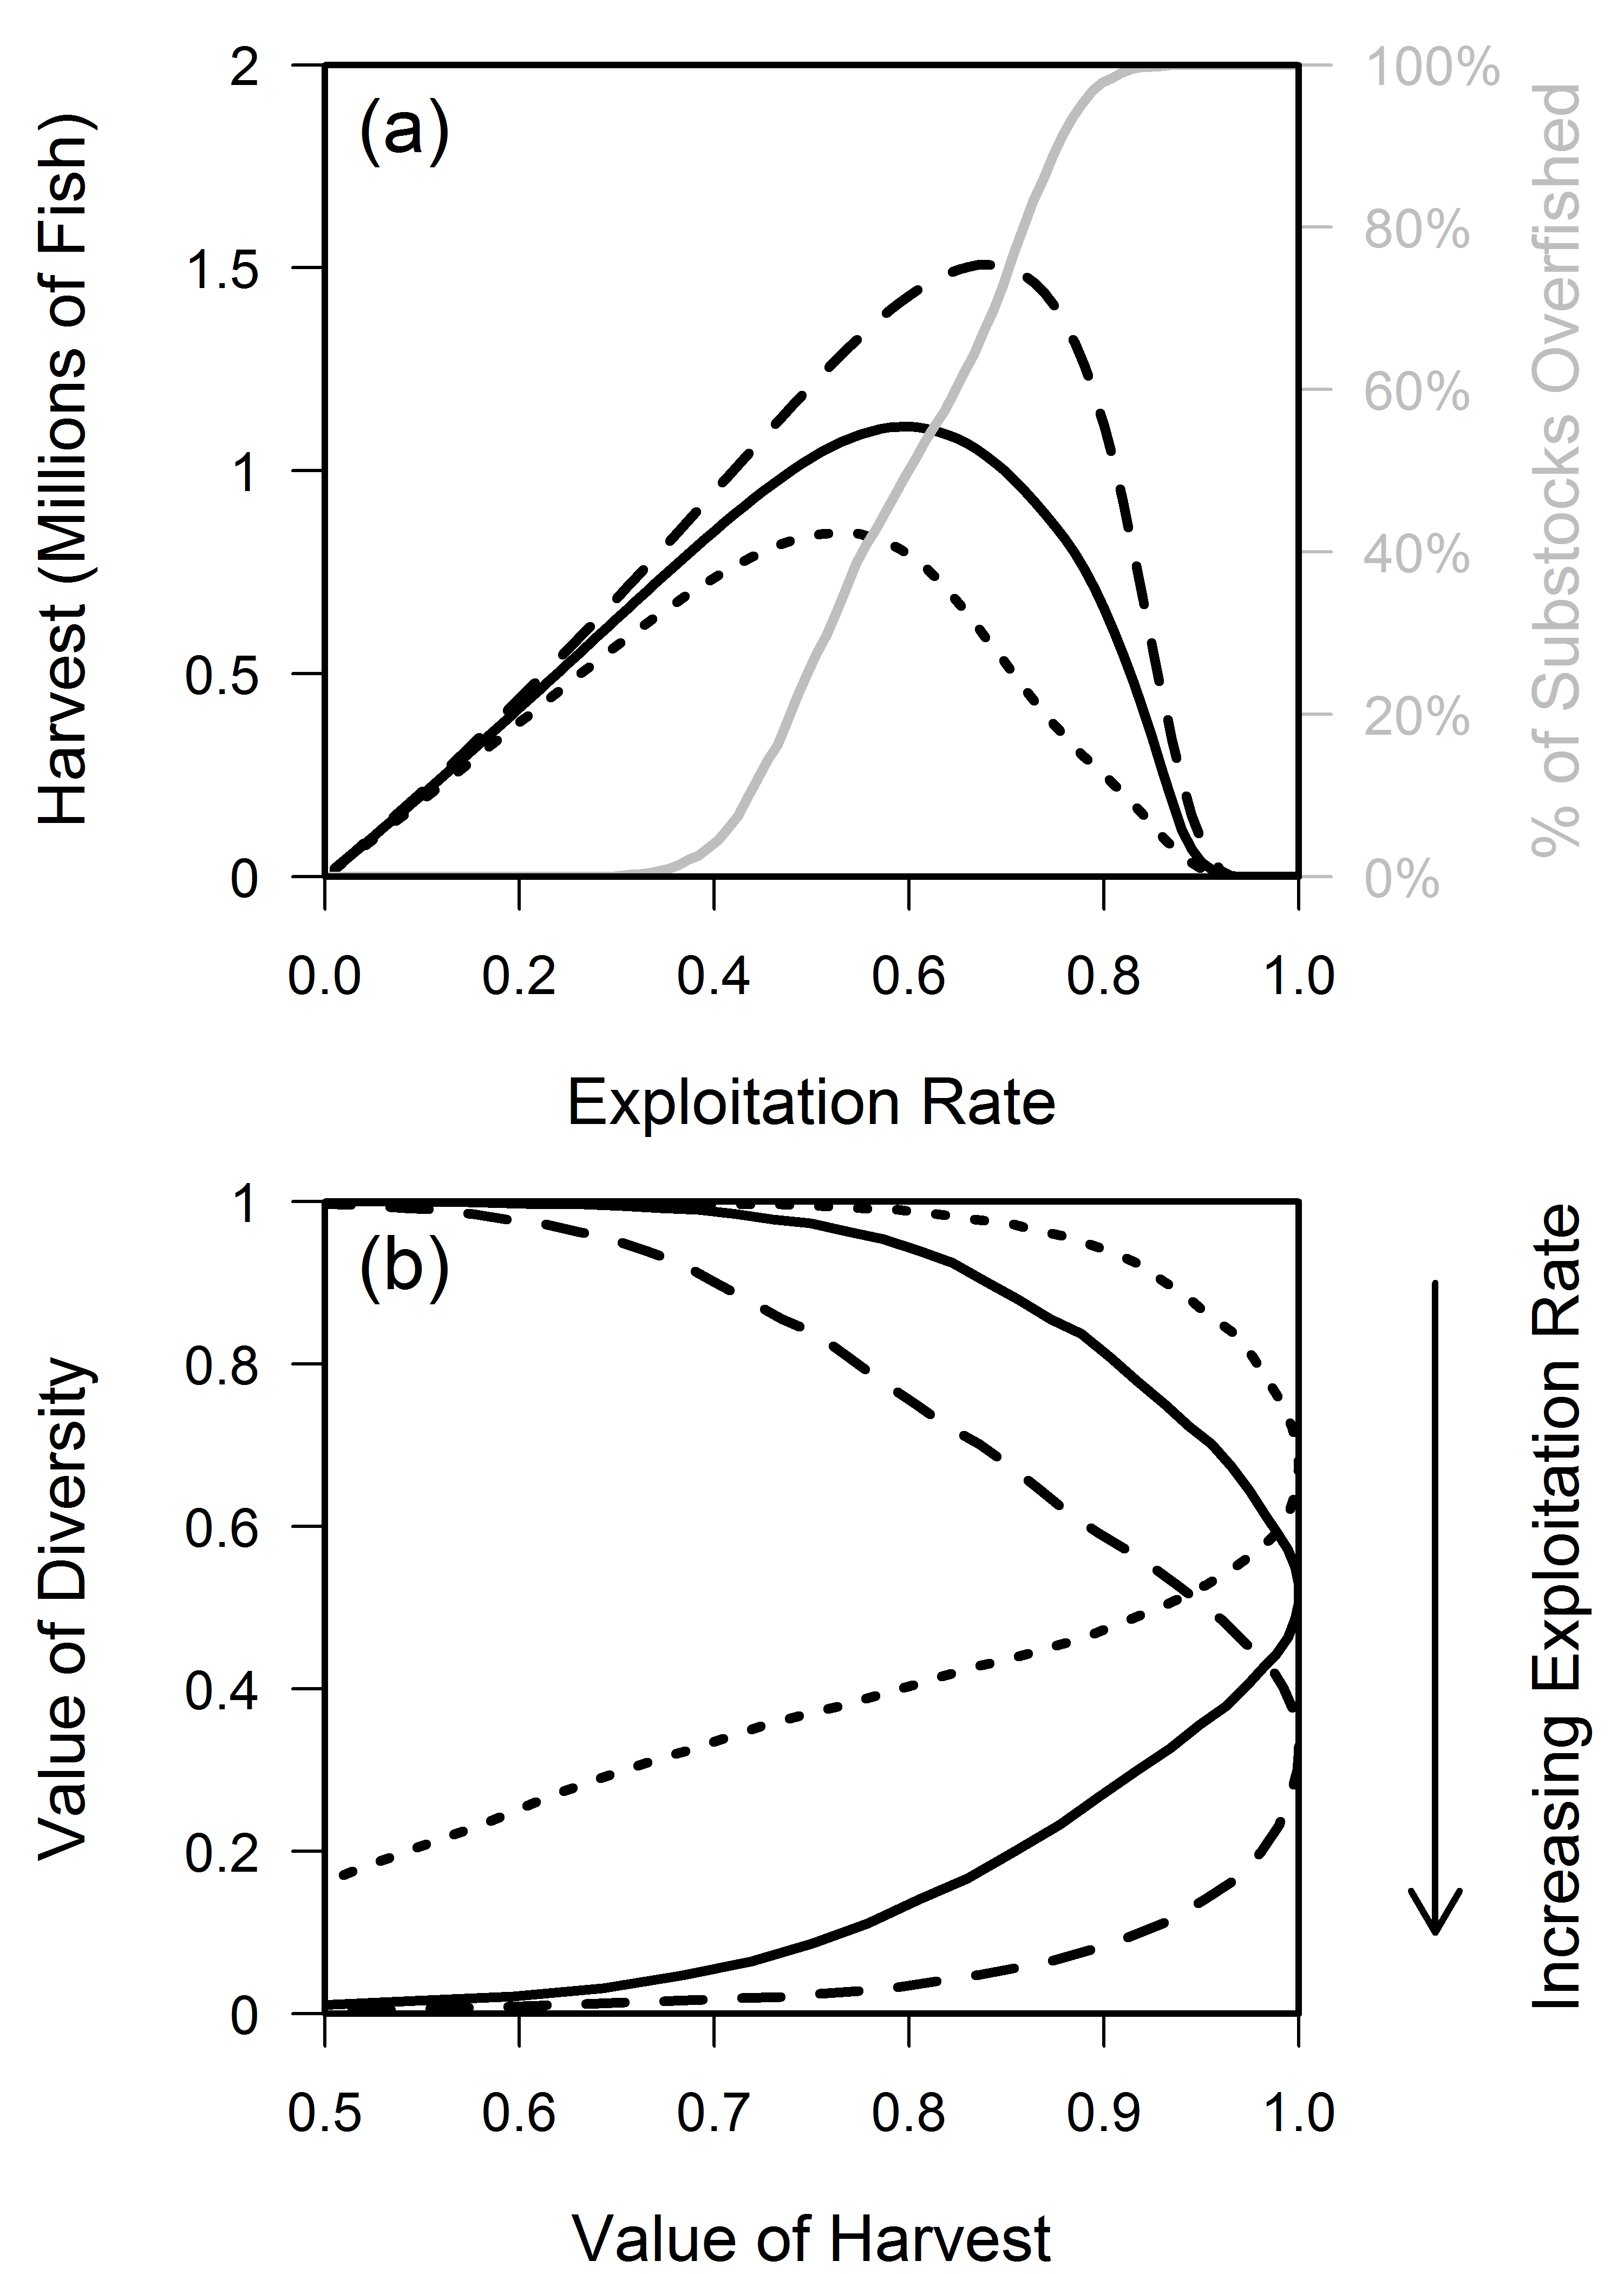
\includegraphics{img/Ch4/trade-off-plot.png}
  \caption{Visualization of how different types of hetergeneity in substock productivity and size influence the shape of trade-offs in mixed-stock salmon fisheries. Solid black likes are the case where stock types are split evenly among large/small and productive/unproductive stocks. Dotted black likes are the case where all small stocks are productive and all large stocks are unproductive, and dashed lines are the opposite (i.e., all big stocks are productive). (\textit{a}) Equilibrium aggregate harvest and proportion of substocks overfished plotted against the exploitation rate (\textit{b}) value of the biodiversity objective (0 = all stocks overfished) plotted against the value of harvest (the long term proportion of the aggregate MSY attained). Notice that when all big stocks are productive (dashed lines), the trade-off is steeper, i.e., more harvest must be sacrificed in order to ensure a greater fraction of substocks are not overfished. }
  \label{fig:trade-off-plot}
\end{figure}

\clearpage

\begin{figure}
  \centering
  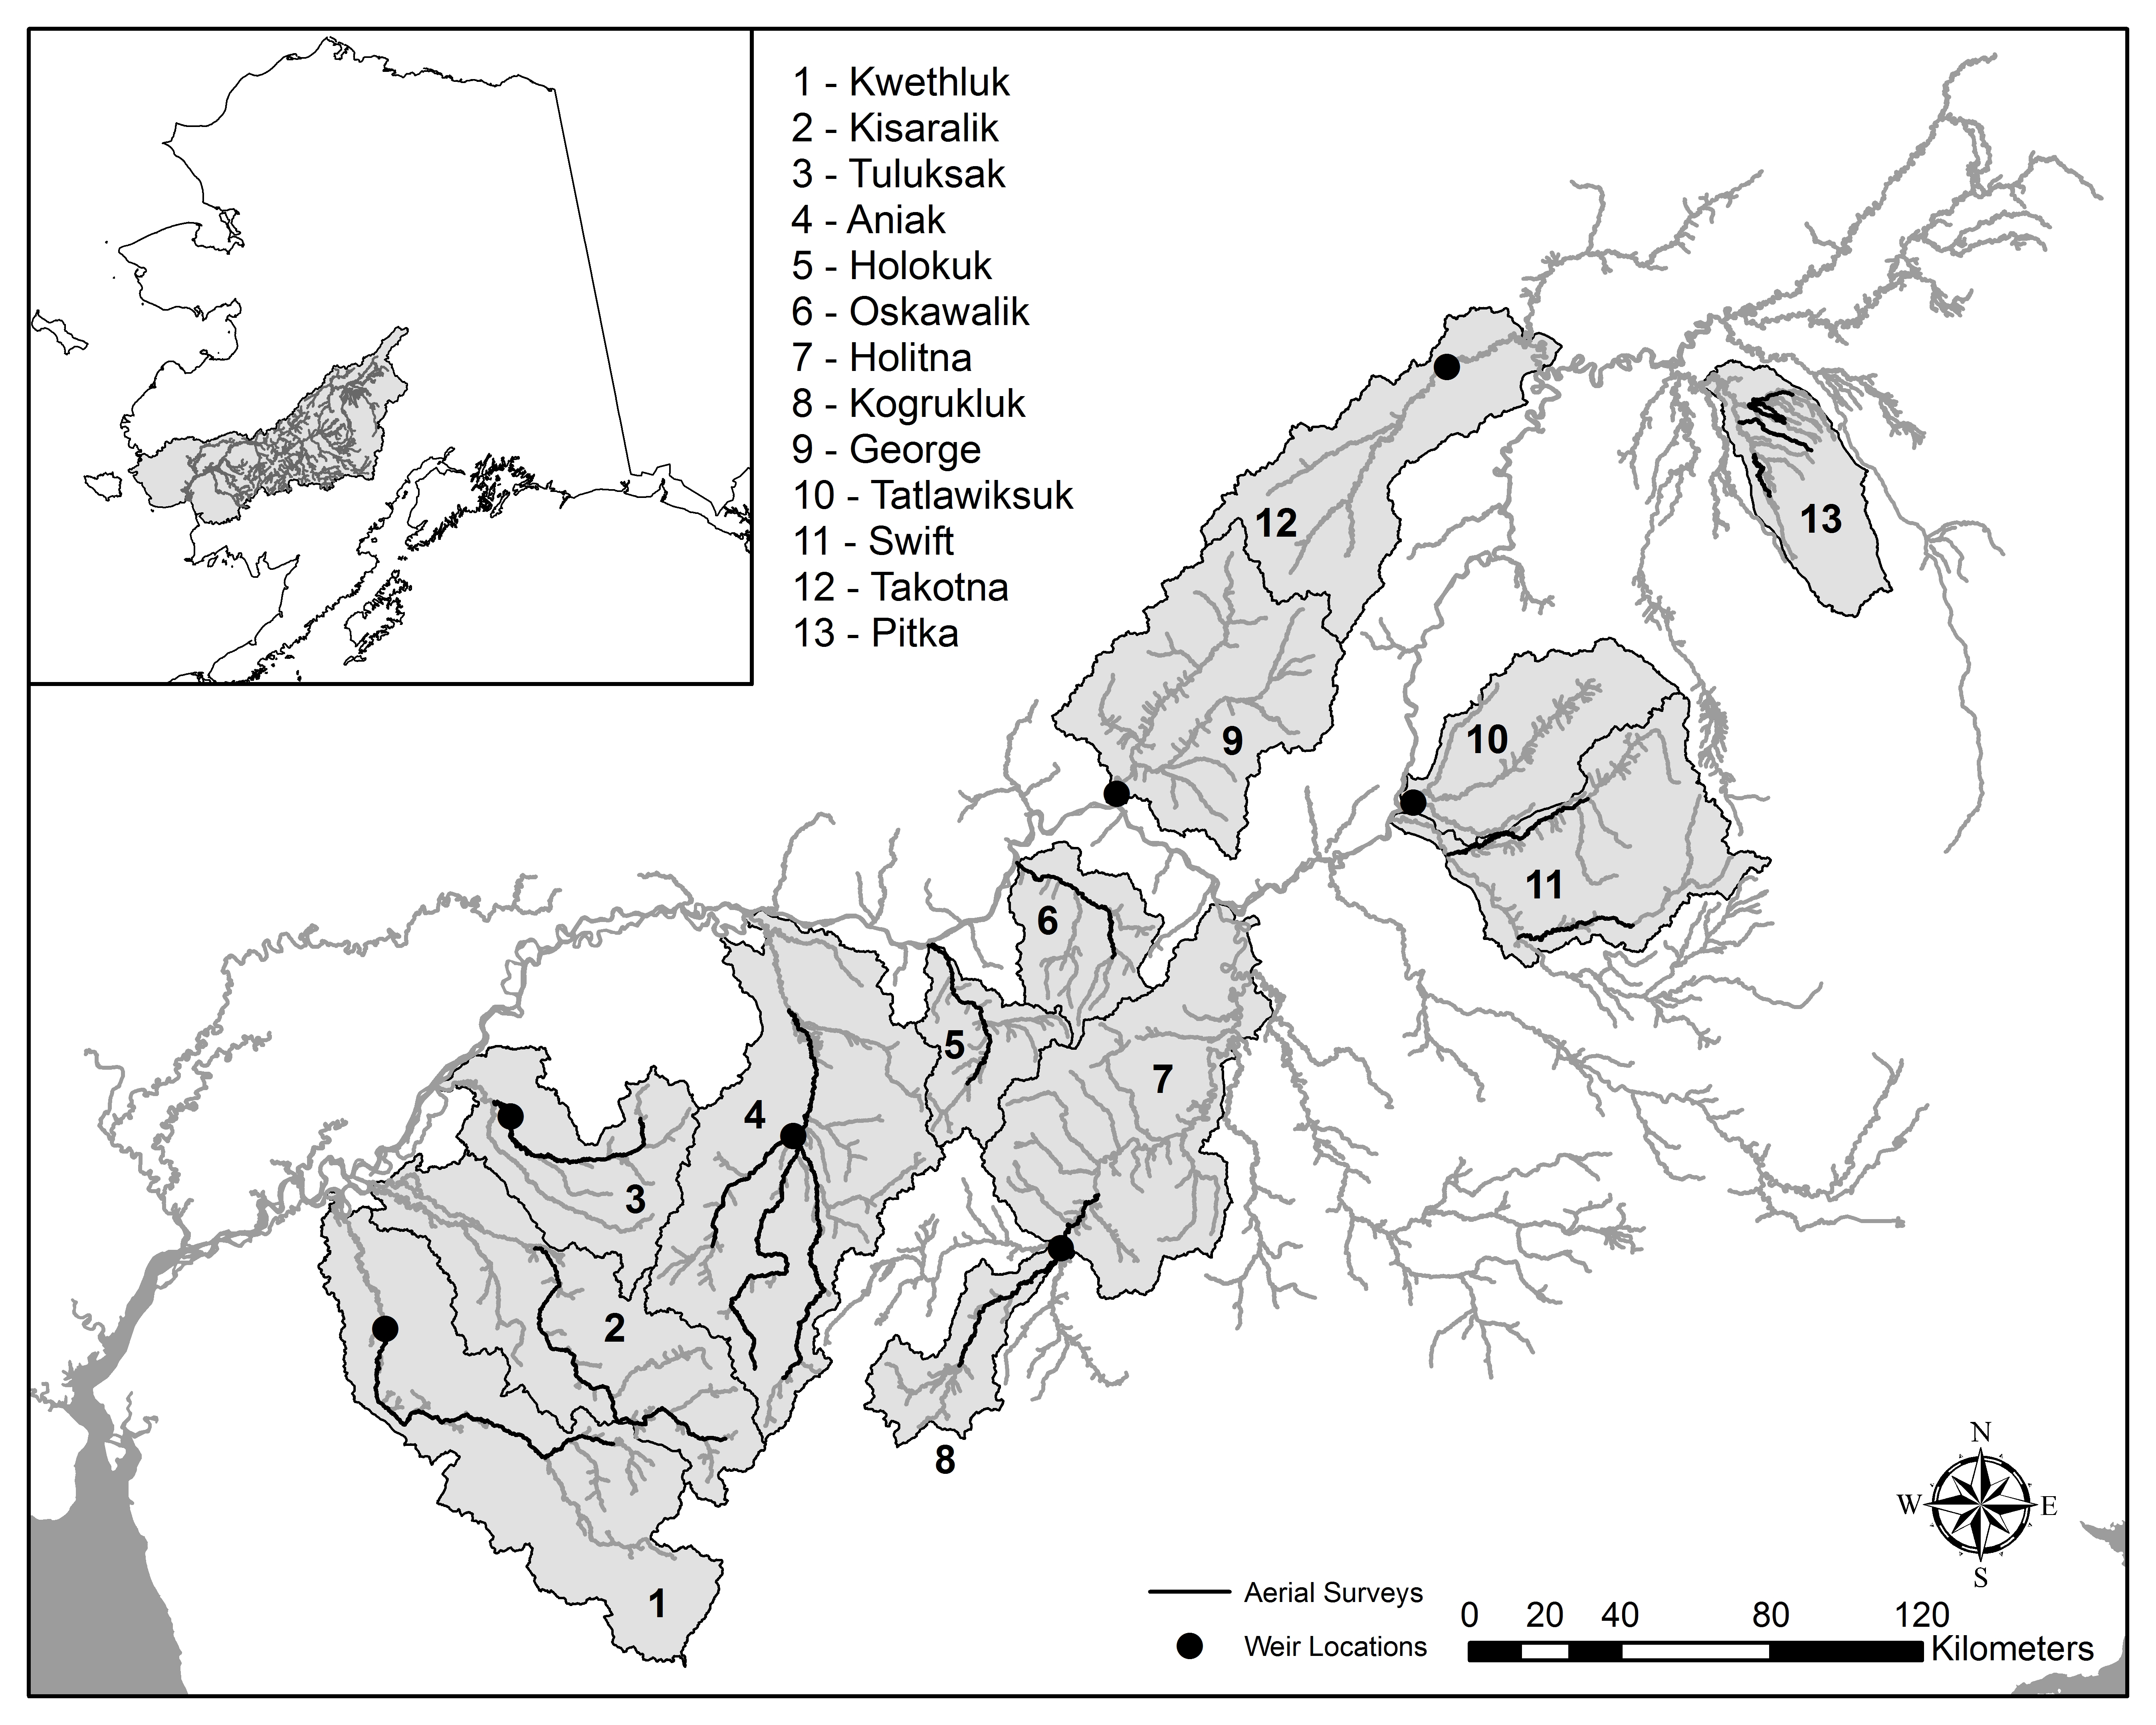
\includegraphics{img/Ch4/ch4-map.jpg}
  \caption{Map of the Kuskokwim River drainage, with the 13 drainage basins representing unique spawning units (substocks) used in this analysis. Black points show the location of weir projects, black sections of river indicate the reaches flown as part of aerial surveys. Drainages monitored via both aerial survey and weir used the weir counts to inform escapement estimates in this analysis, with the exception of the Aniak drainage (4), for which aerial survey data were much more abundant than the weir data.}
  \label{fig:ch4-map}
\end{figure}

\clearpage

\begin{figure}
  \centering
  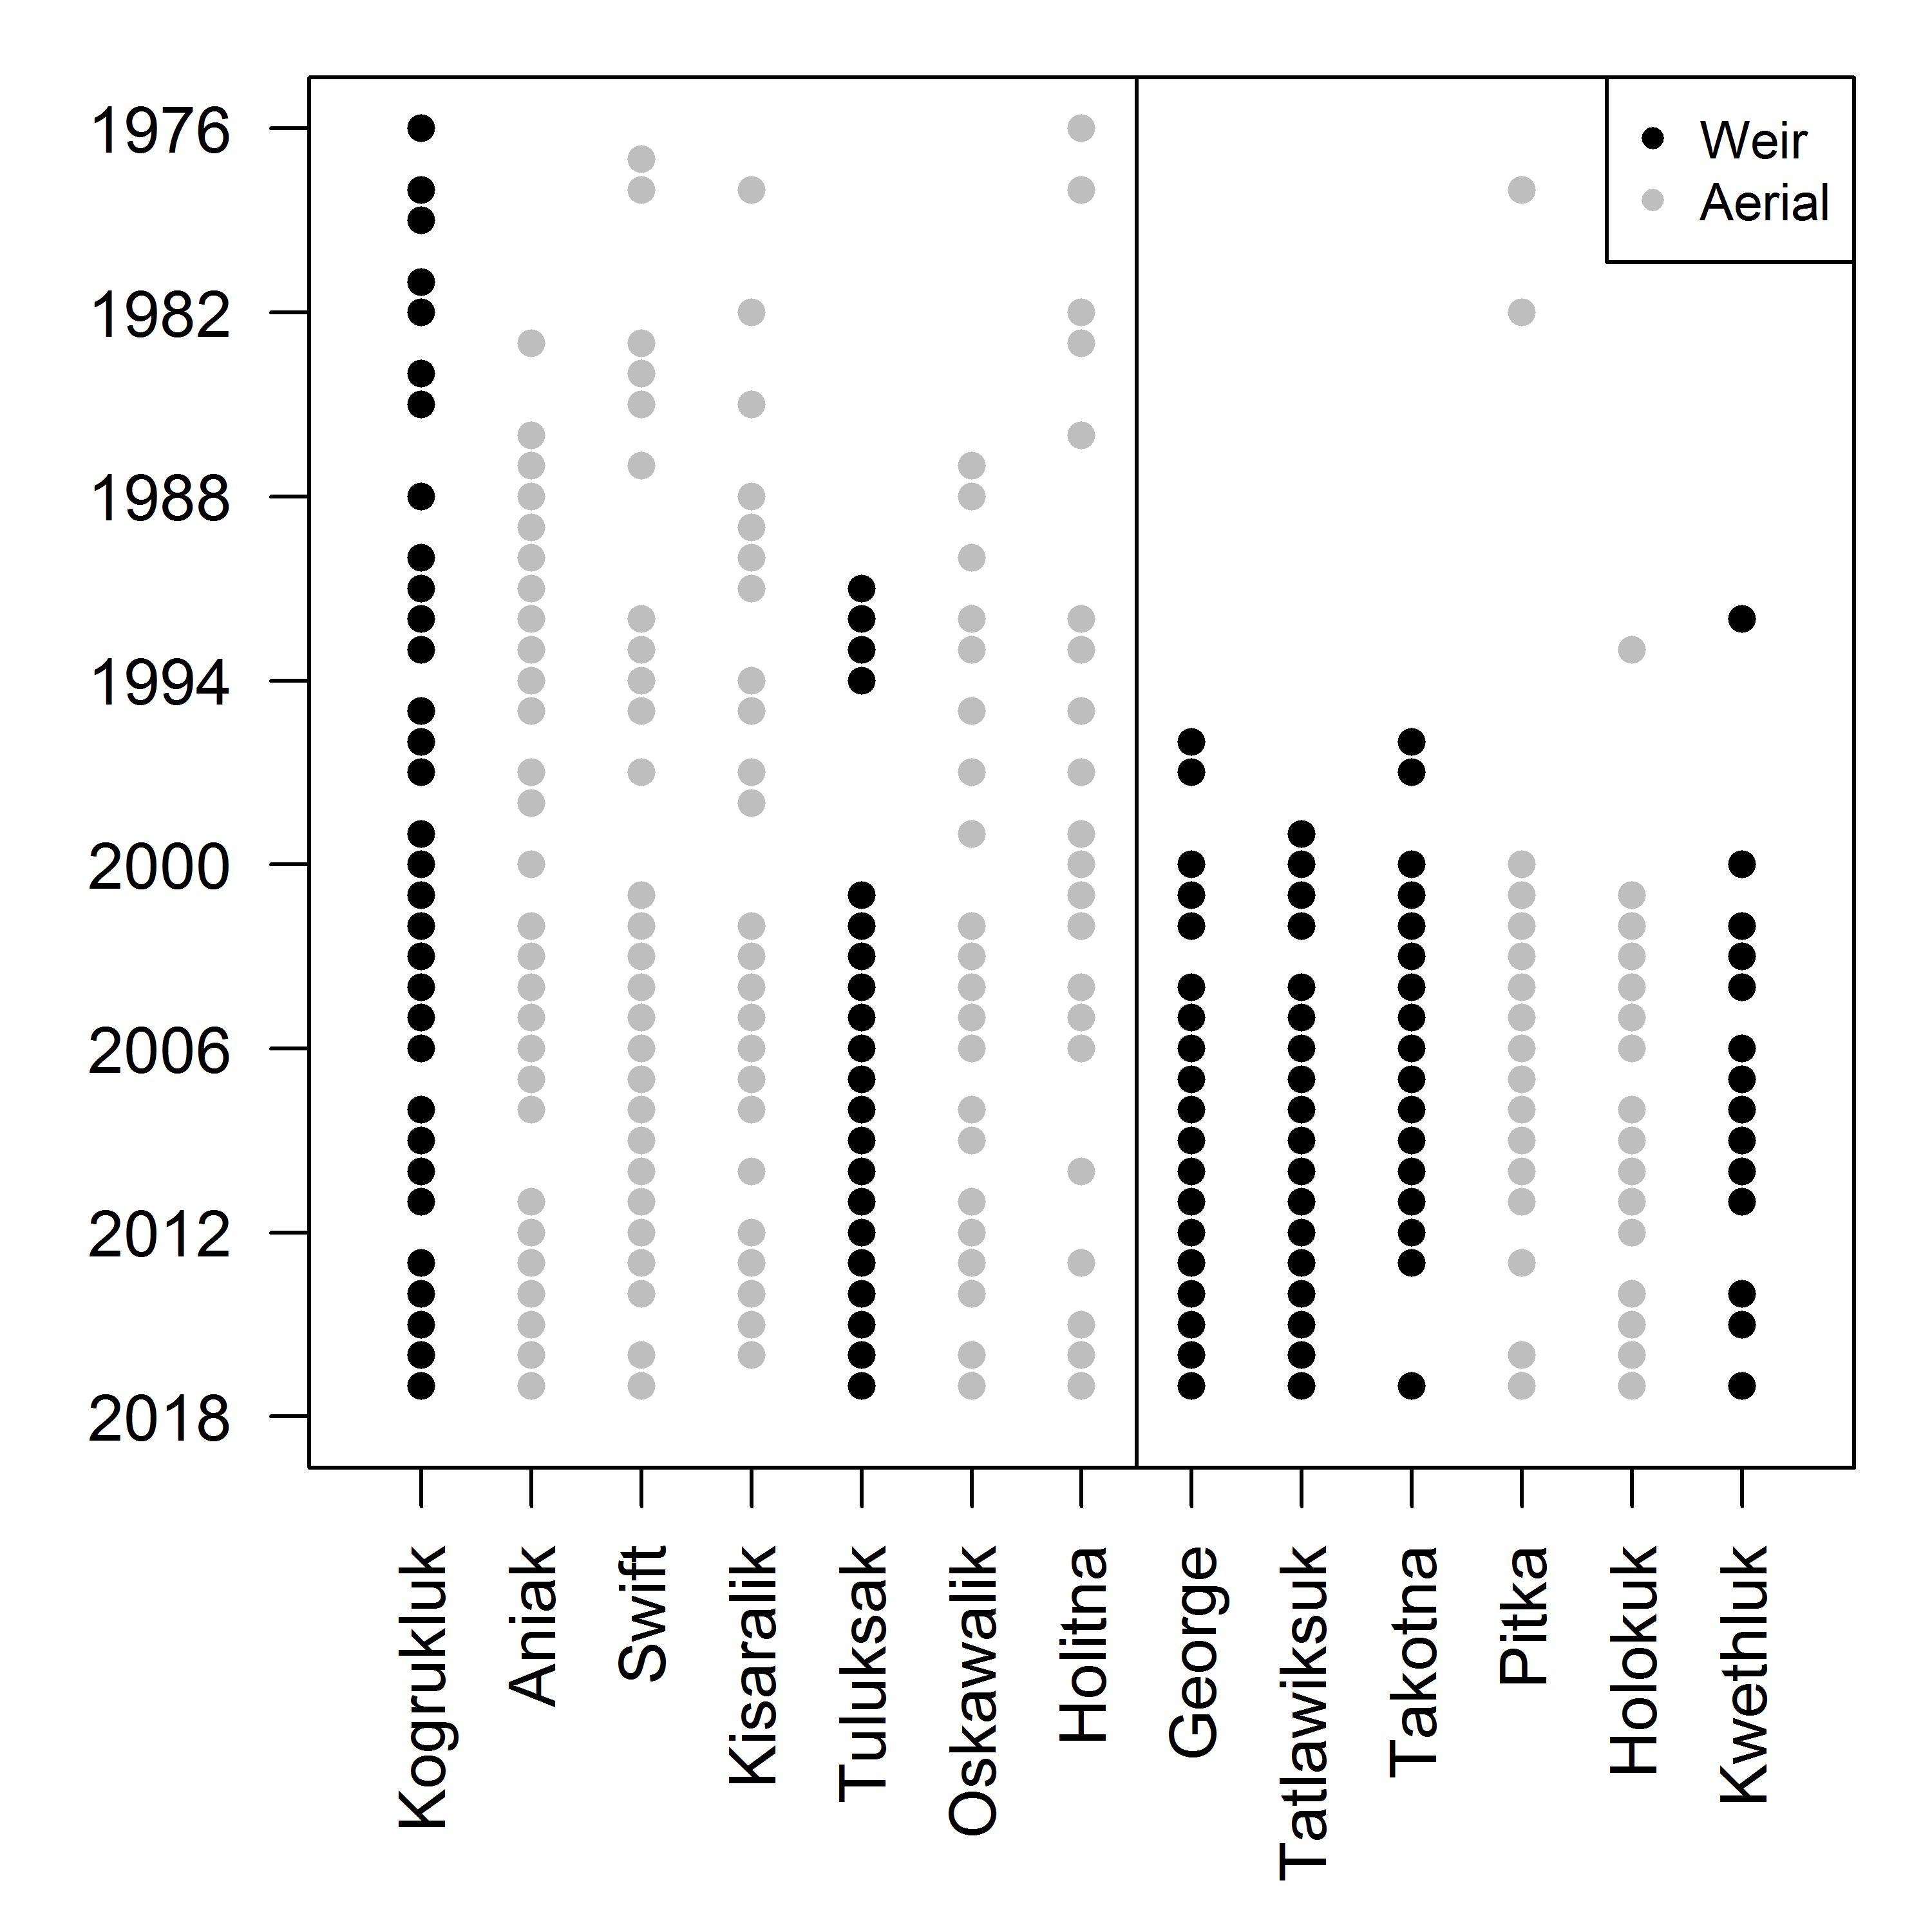
\includegraphics{img/Ch4/obs-freq.jpg}
  \caption{The frequency of escapement sampling for each substock sampled in the Kuskokwim River. Black points indicate years that were sampled for substocks monitored with a weir and grey points indicate years sampled for substocks monitored with aerial surveys. The vertical black line shows a break where > 50\% of the years were monitored for a stock.}
  \label{fig:obs-freq}
\end{figure}

\clearpage

\begin{figure}
  \centering
  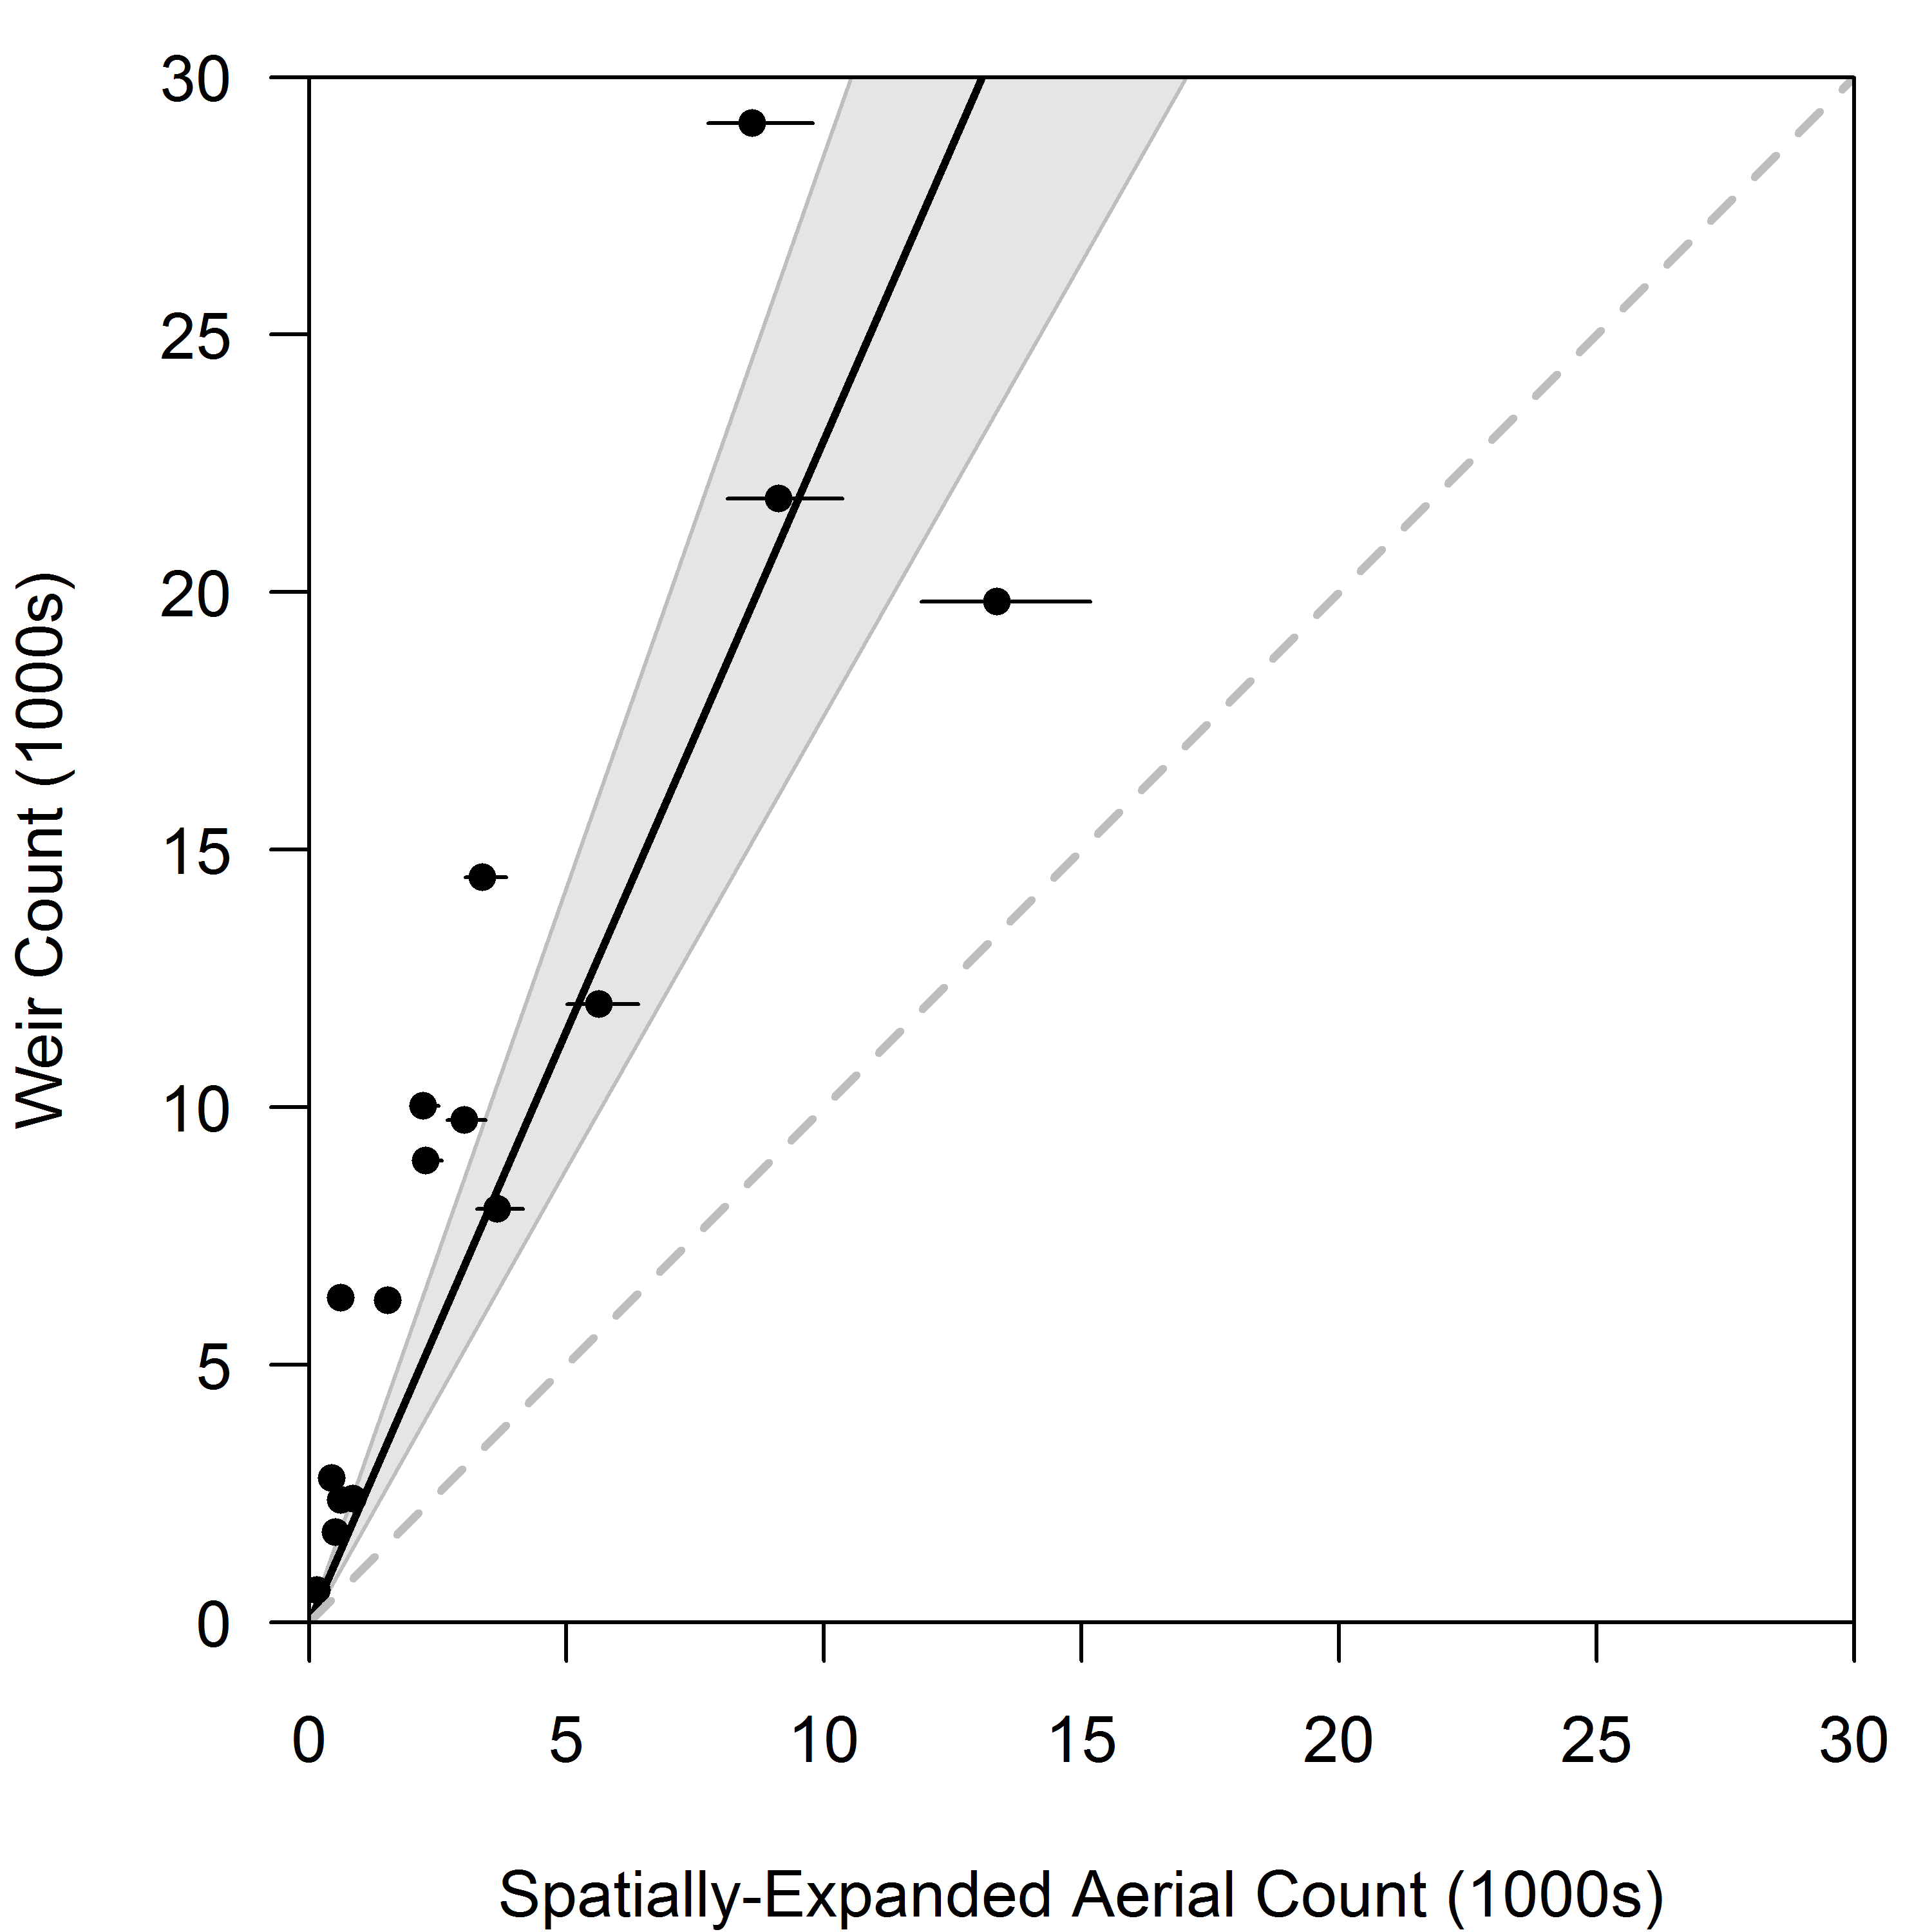
\includegraphics{img/Ch4/obs-correct.png}
  \caption{The relationship between spatially-expanded aerial survey estimates and weir counts during the same years and substocks as described by (\ref{eq:temp-expand1}). Notice the uncertainty expressed in the predictor variable; this was included in the analysis by incorporating both the spatial (Section \ref{spat-expansion}) and temporal (Section \ref{temp-expansion}) expansions in a single model fitted using Bayesian methods.}
  \label{fig:obs-correct}
\end{figure}

\clearpage

\begin{figure}
  \centering
  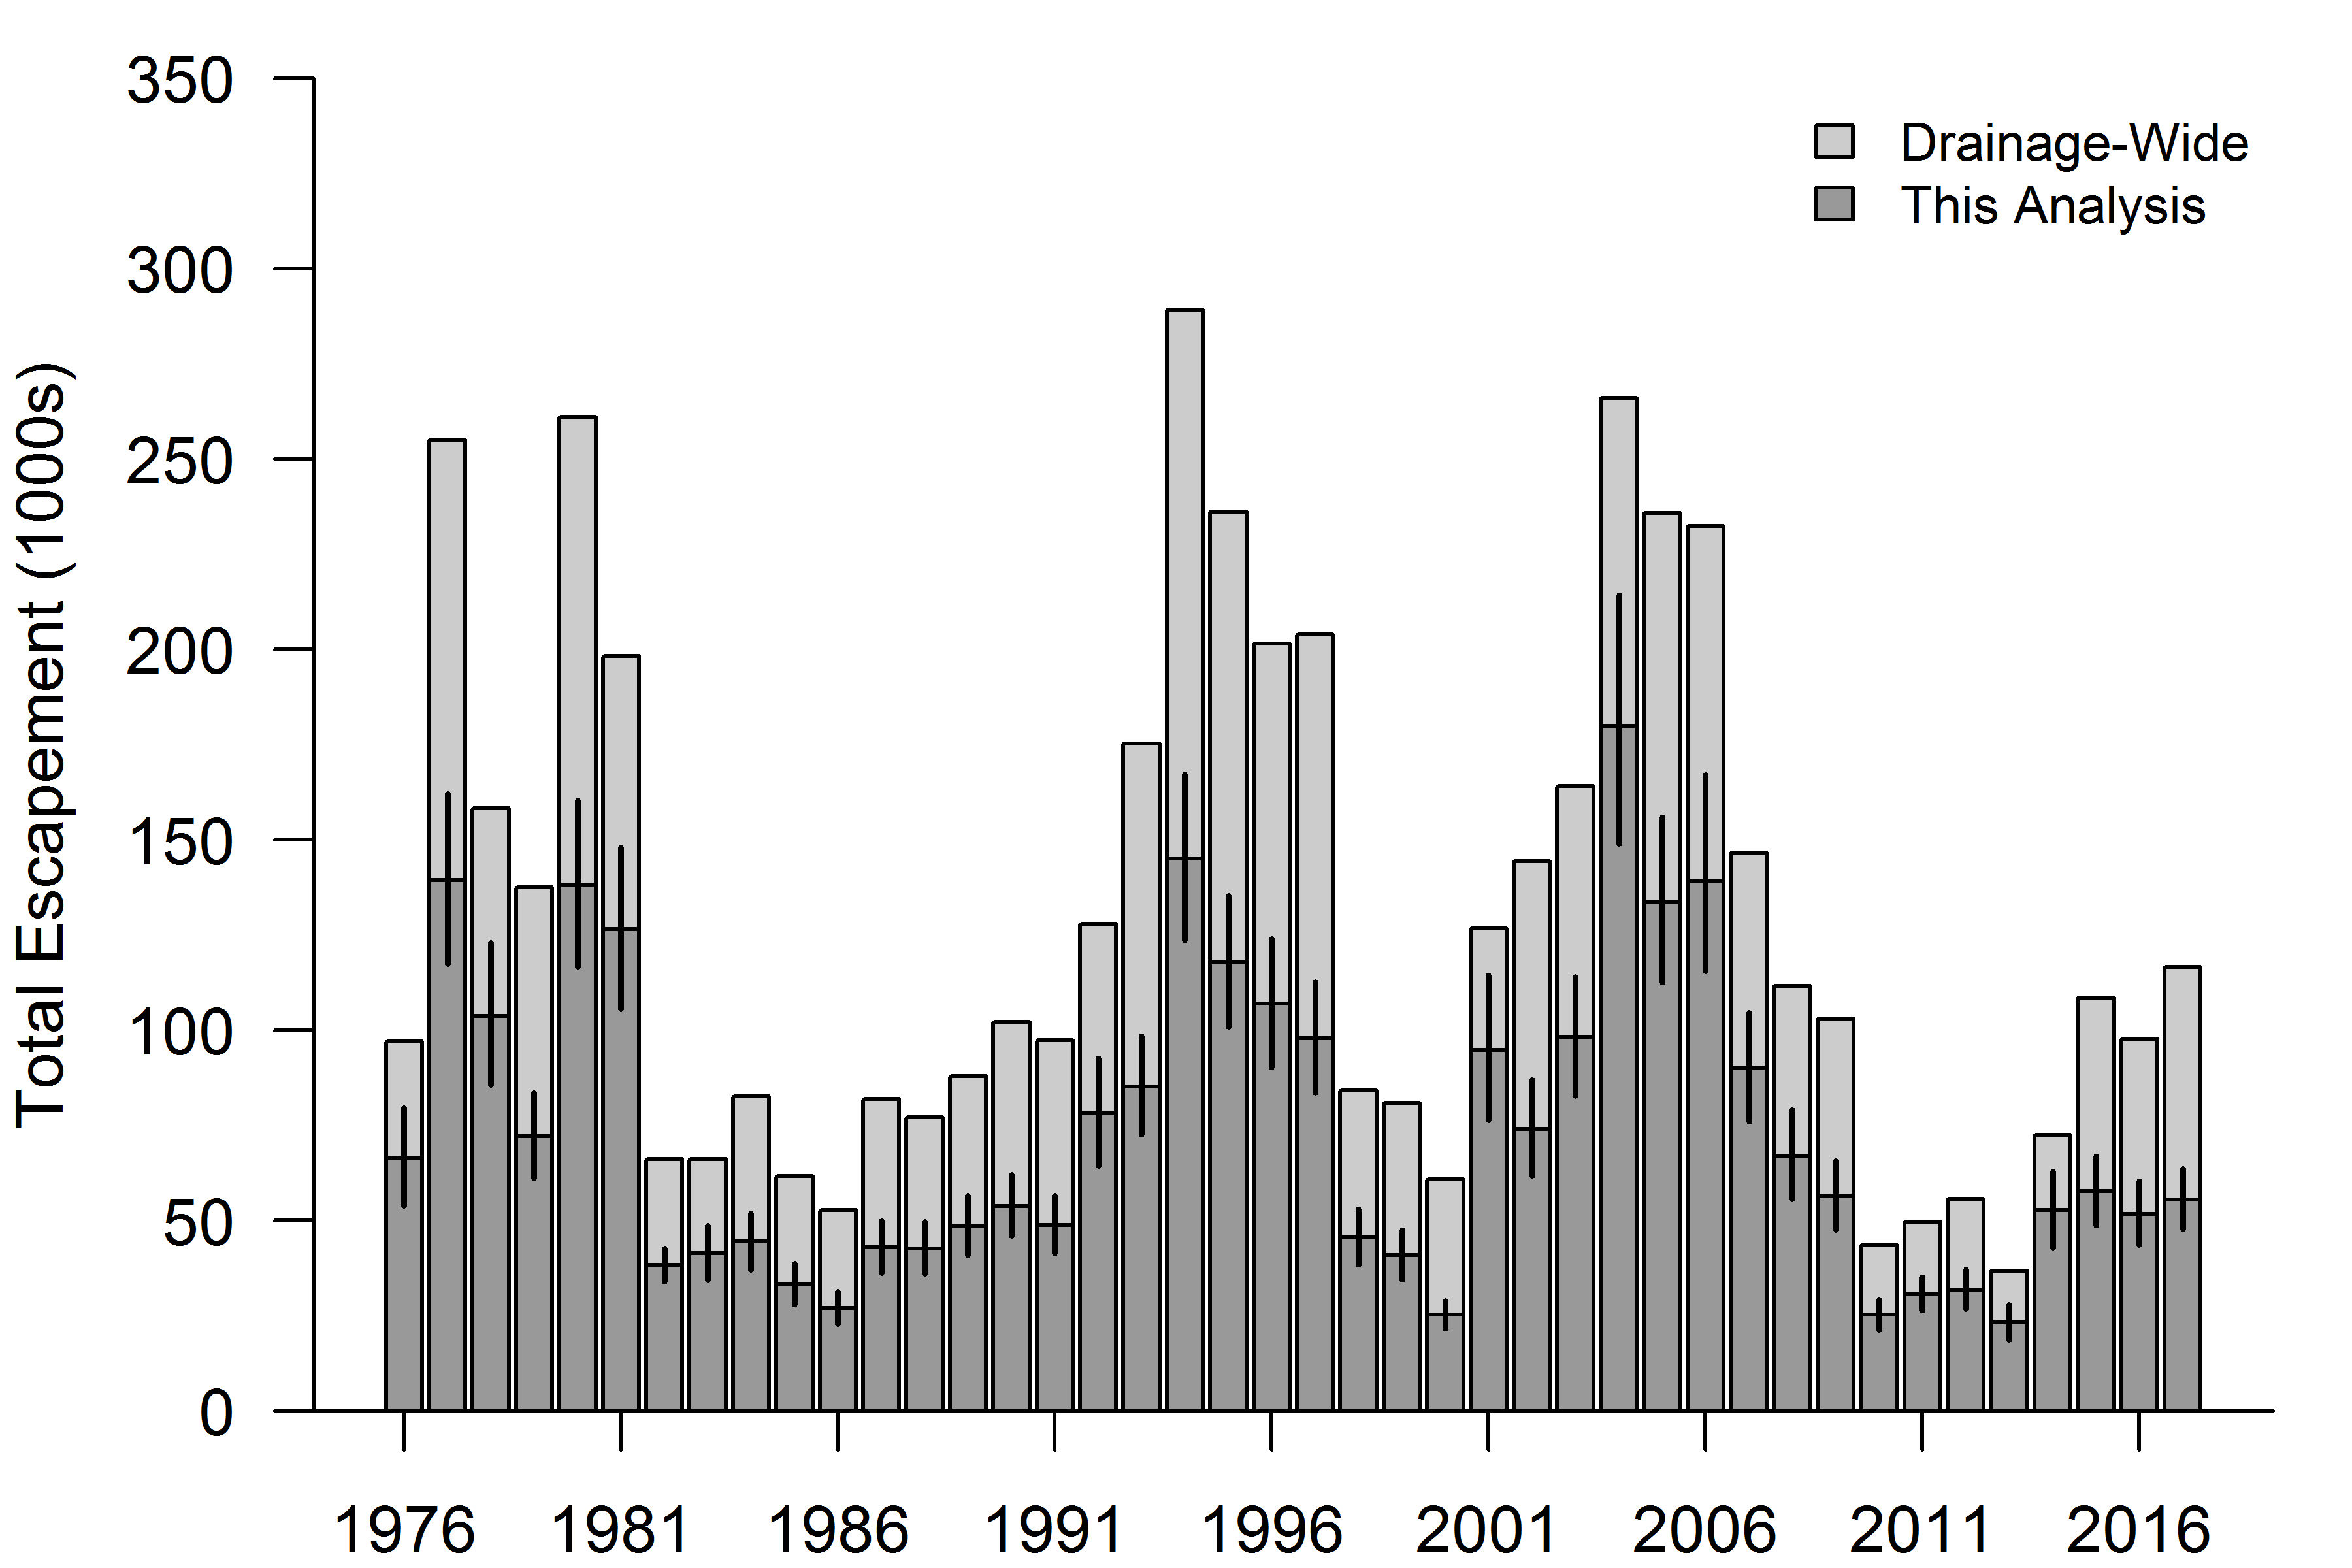
\includegraphics{img/Ch4/obs-fraction.png}
  \caption{Estimated Chinook salmon escapement for substocks within the Kuskokwim River drainage. `Drainage-wide' refers to the aggregate population estimates provided by a maximum likelihood run reconstruction model. `This analysis' refers to the estimated portion of the aggregate run included in this analysis (not all tributaries have been monitored).}
  \label{fig:obs-fraction}
\end{figure}

\clearpage

\begin{figure}
  \centering
  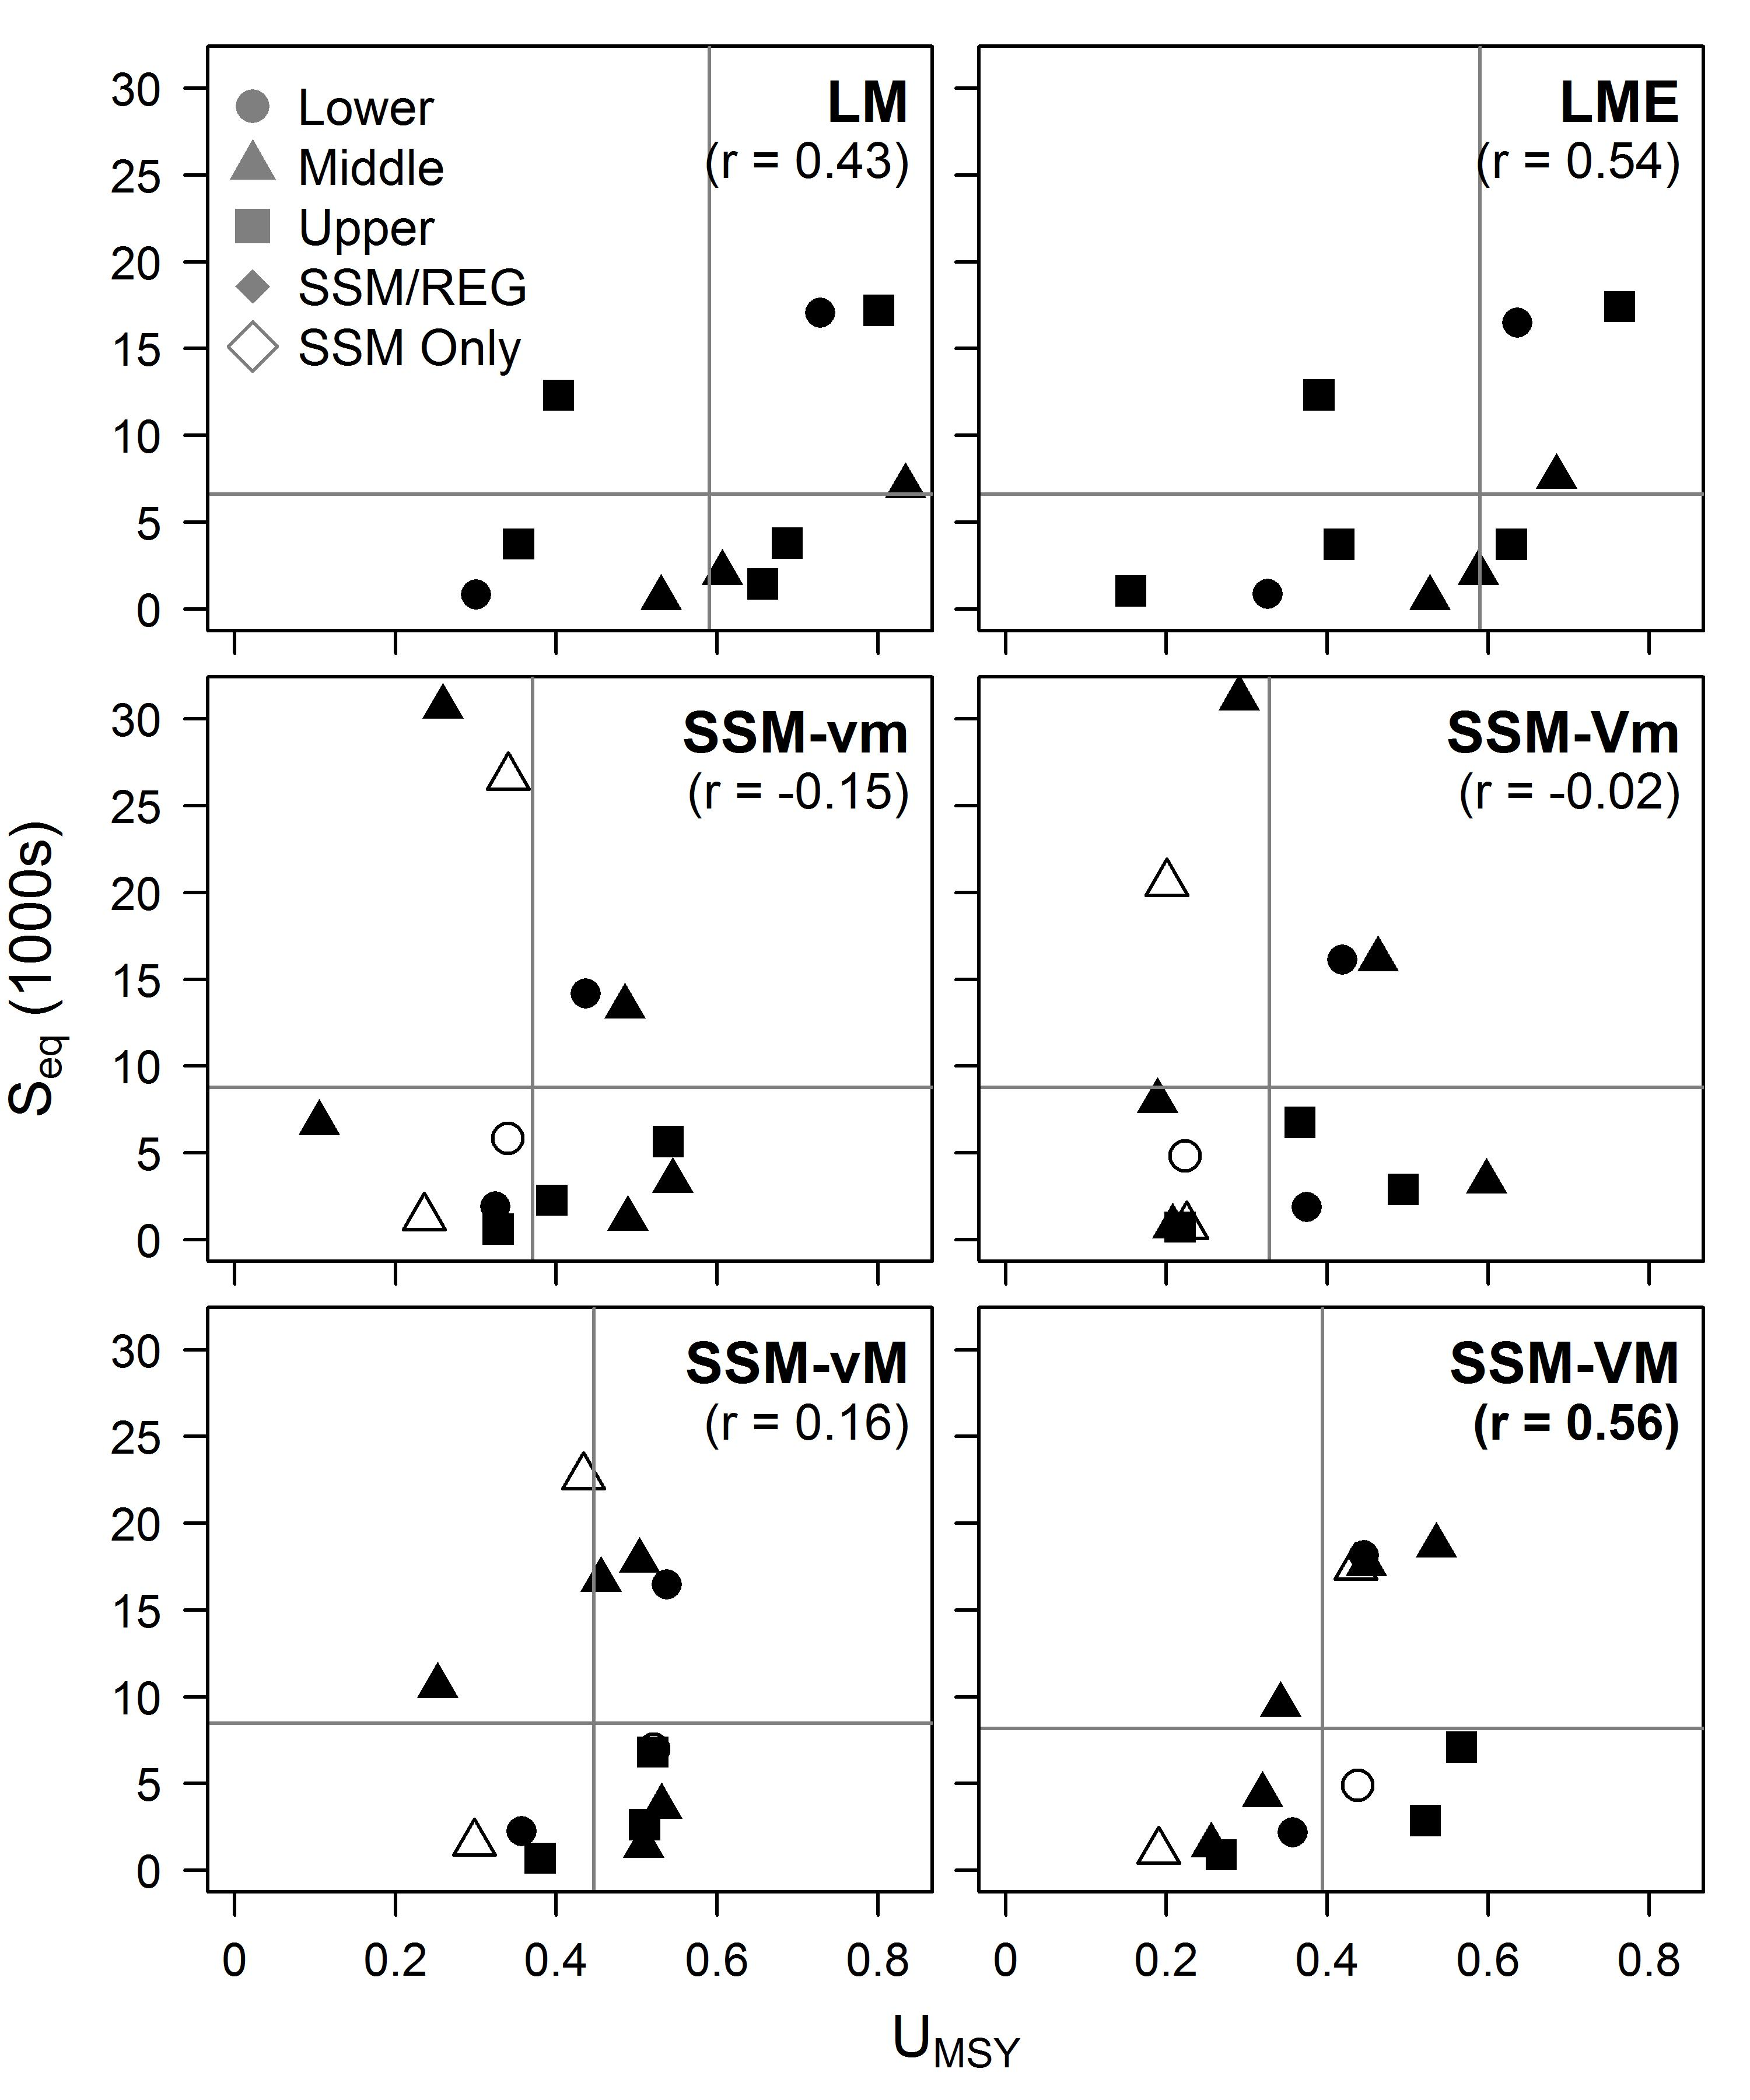
\includegraphics{img/Ch4/Size-v-Prod.jpg}
  \caption{Caption goes here.}
  \label{fig:size-v-prod}
\end{figure}

\clearpage

\begin{figure}
  \centering
  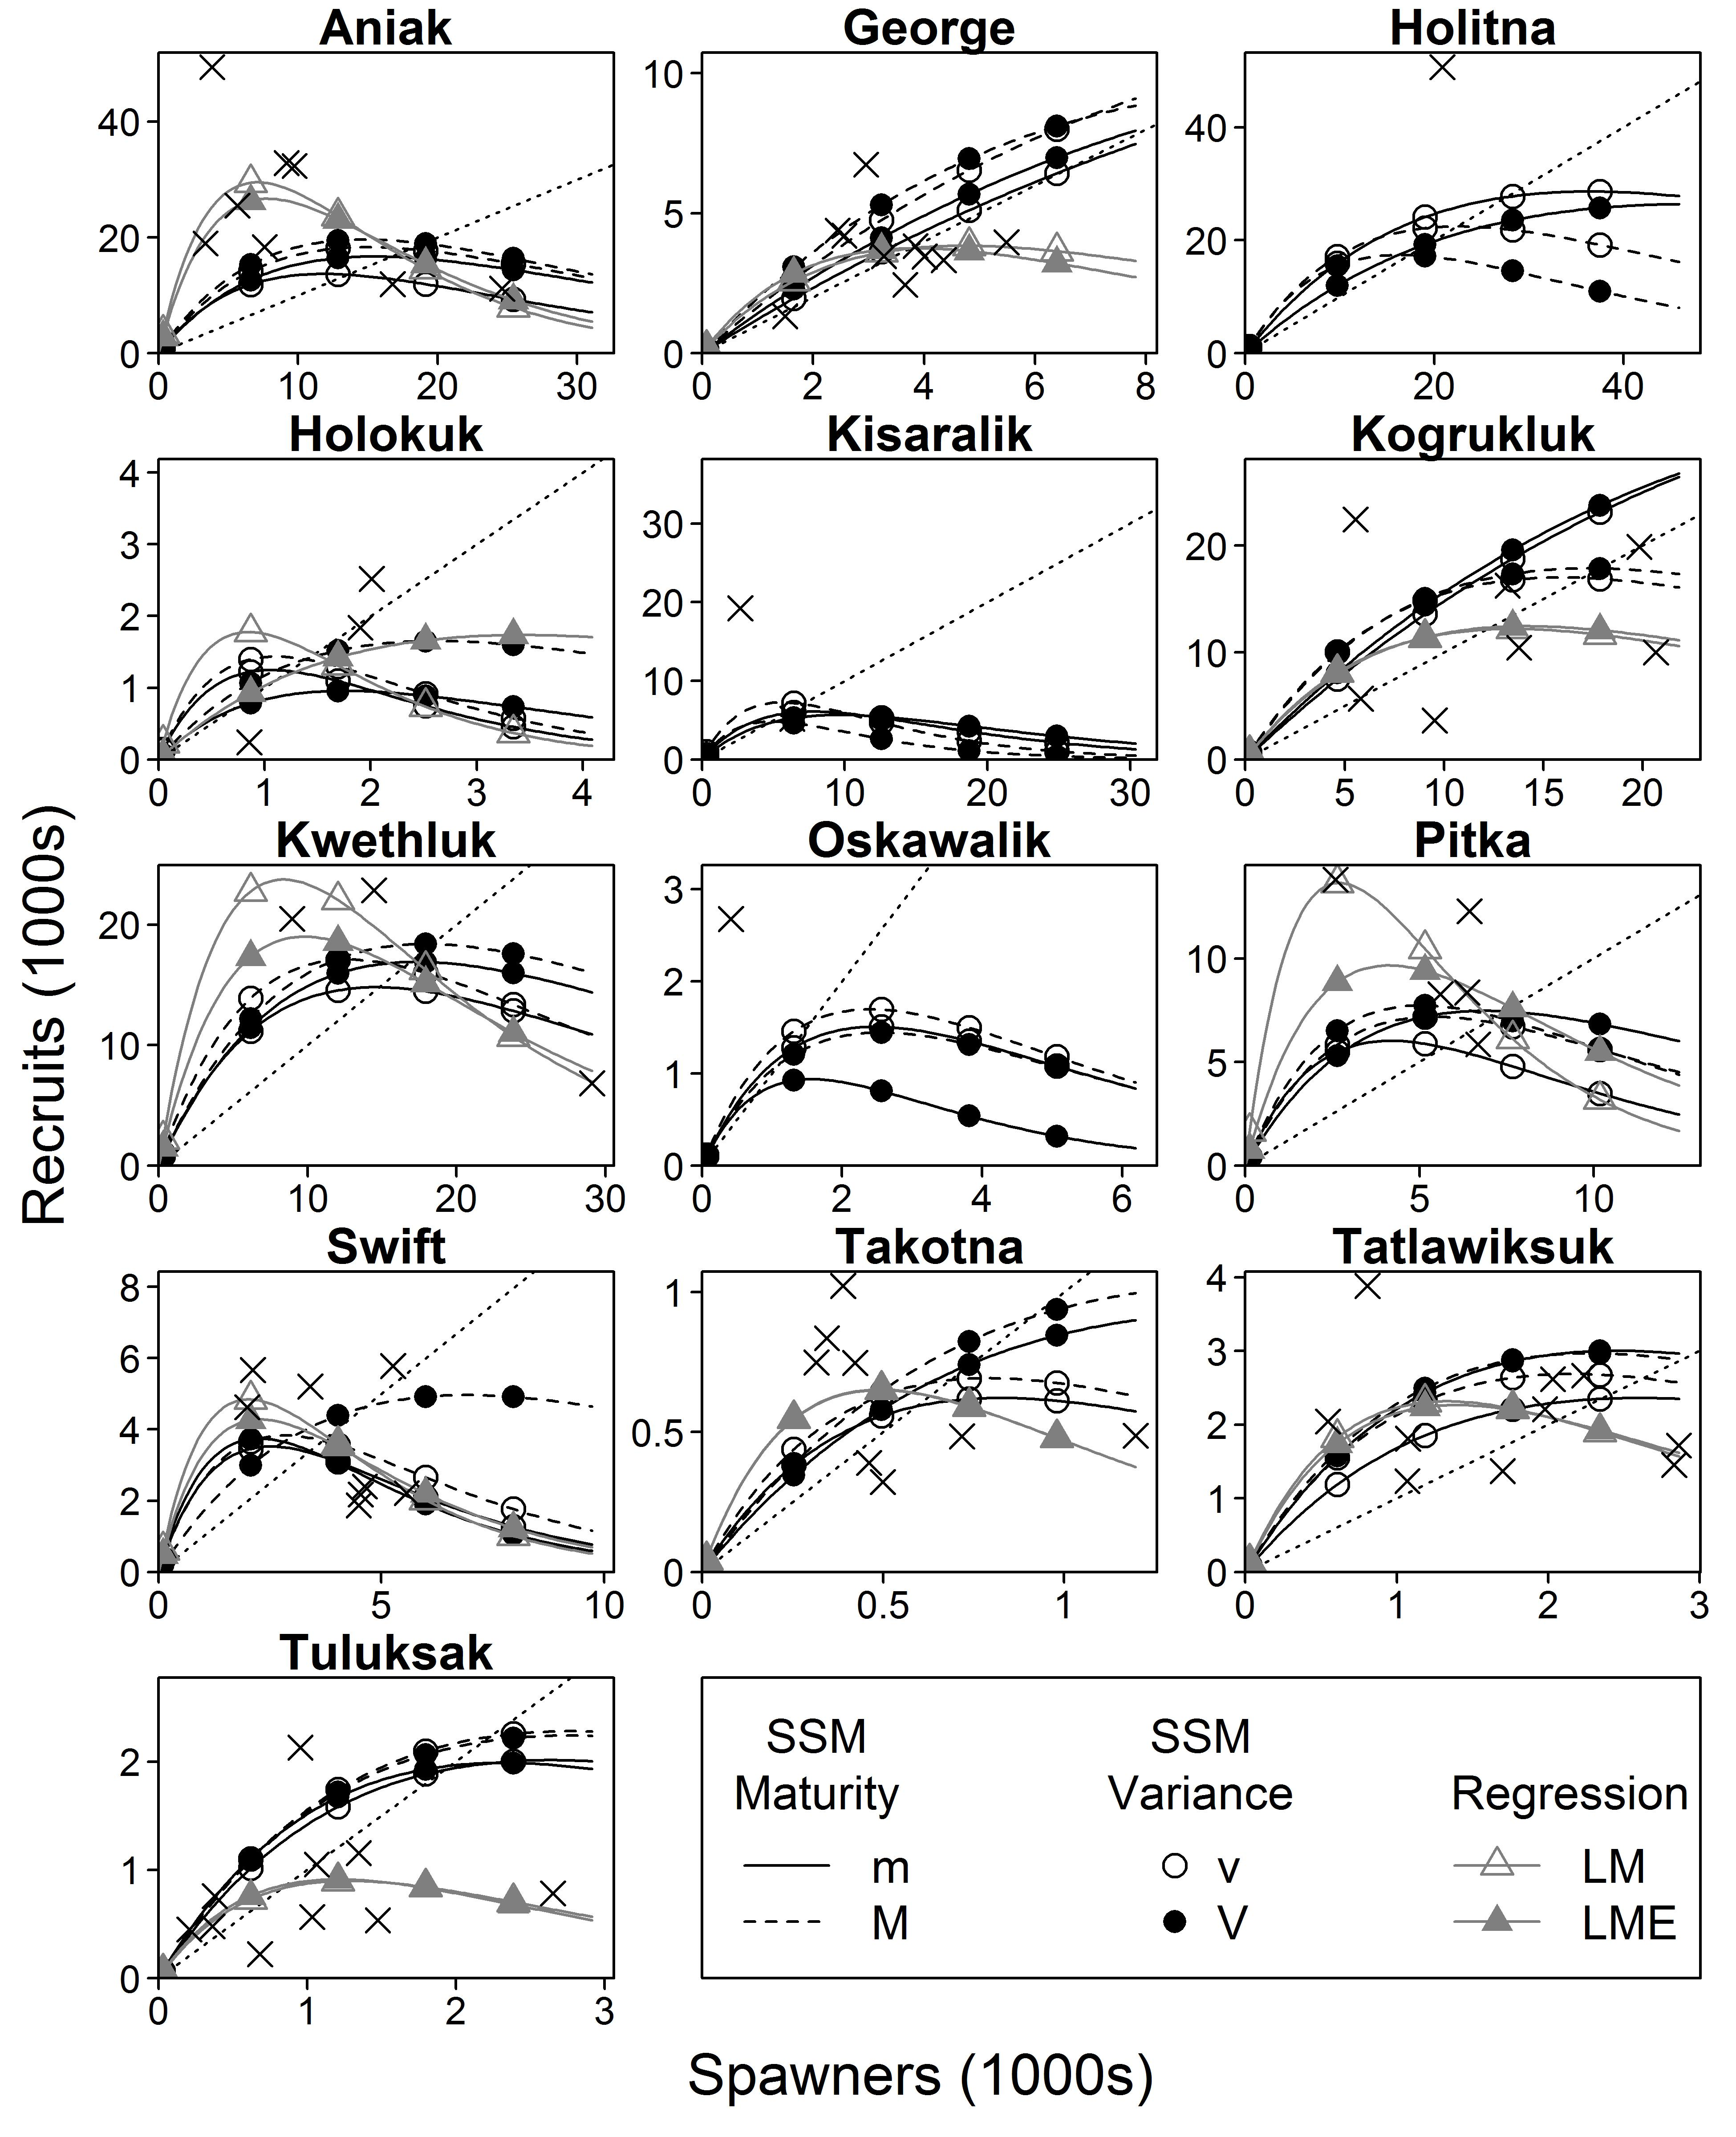
\includegraphics{img/Ch4/R-v-S.jpg}
  \caption{Caption goes here.}
  \label{fig:r-v-s}
\end{figure}

\clearpage

\begin{figure}
  \centering
  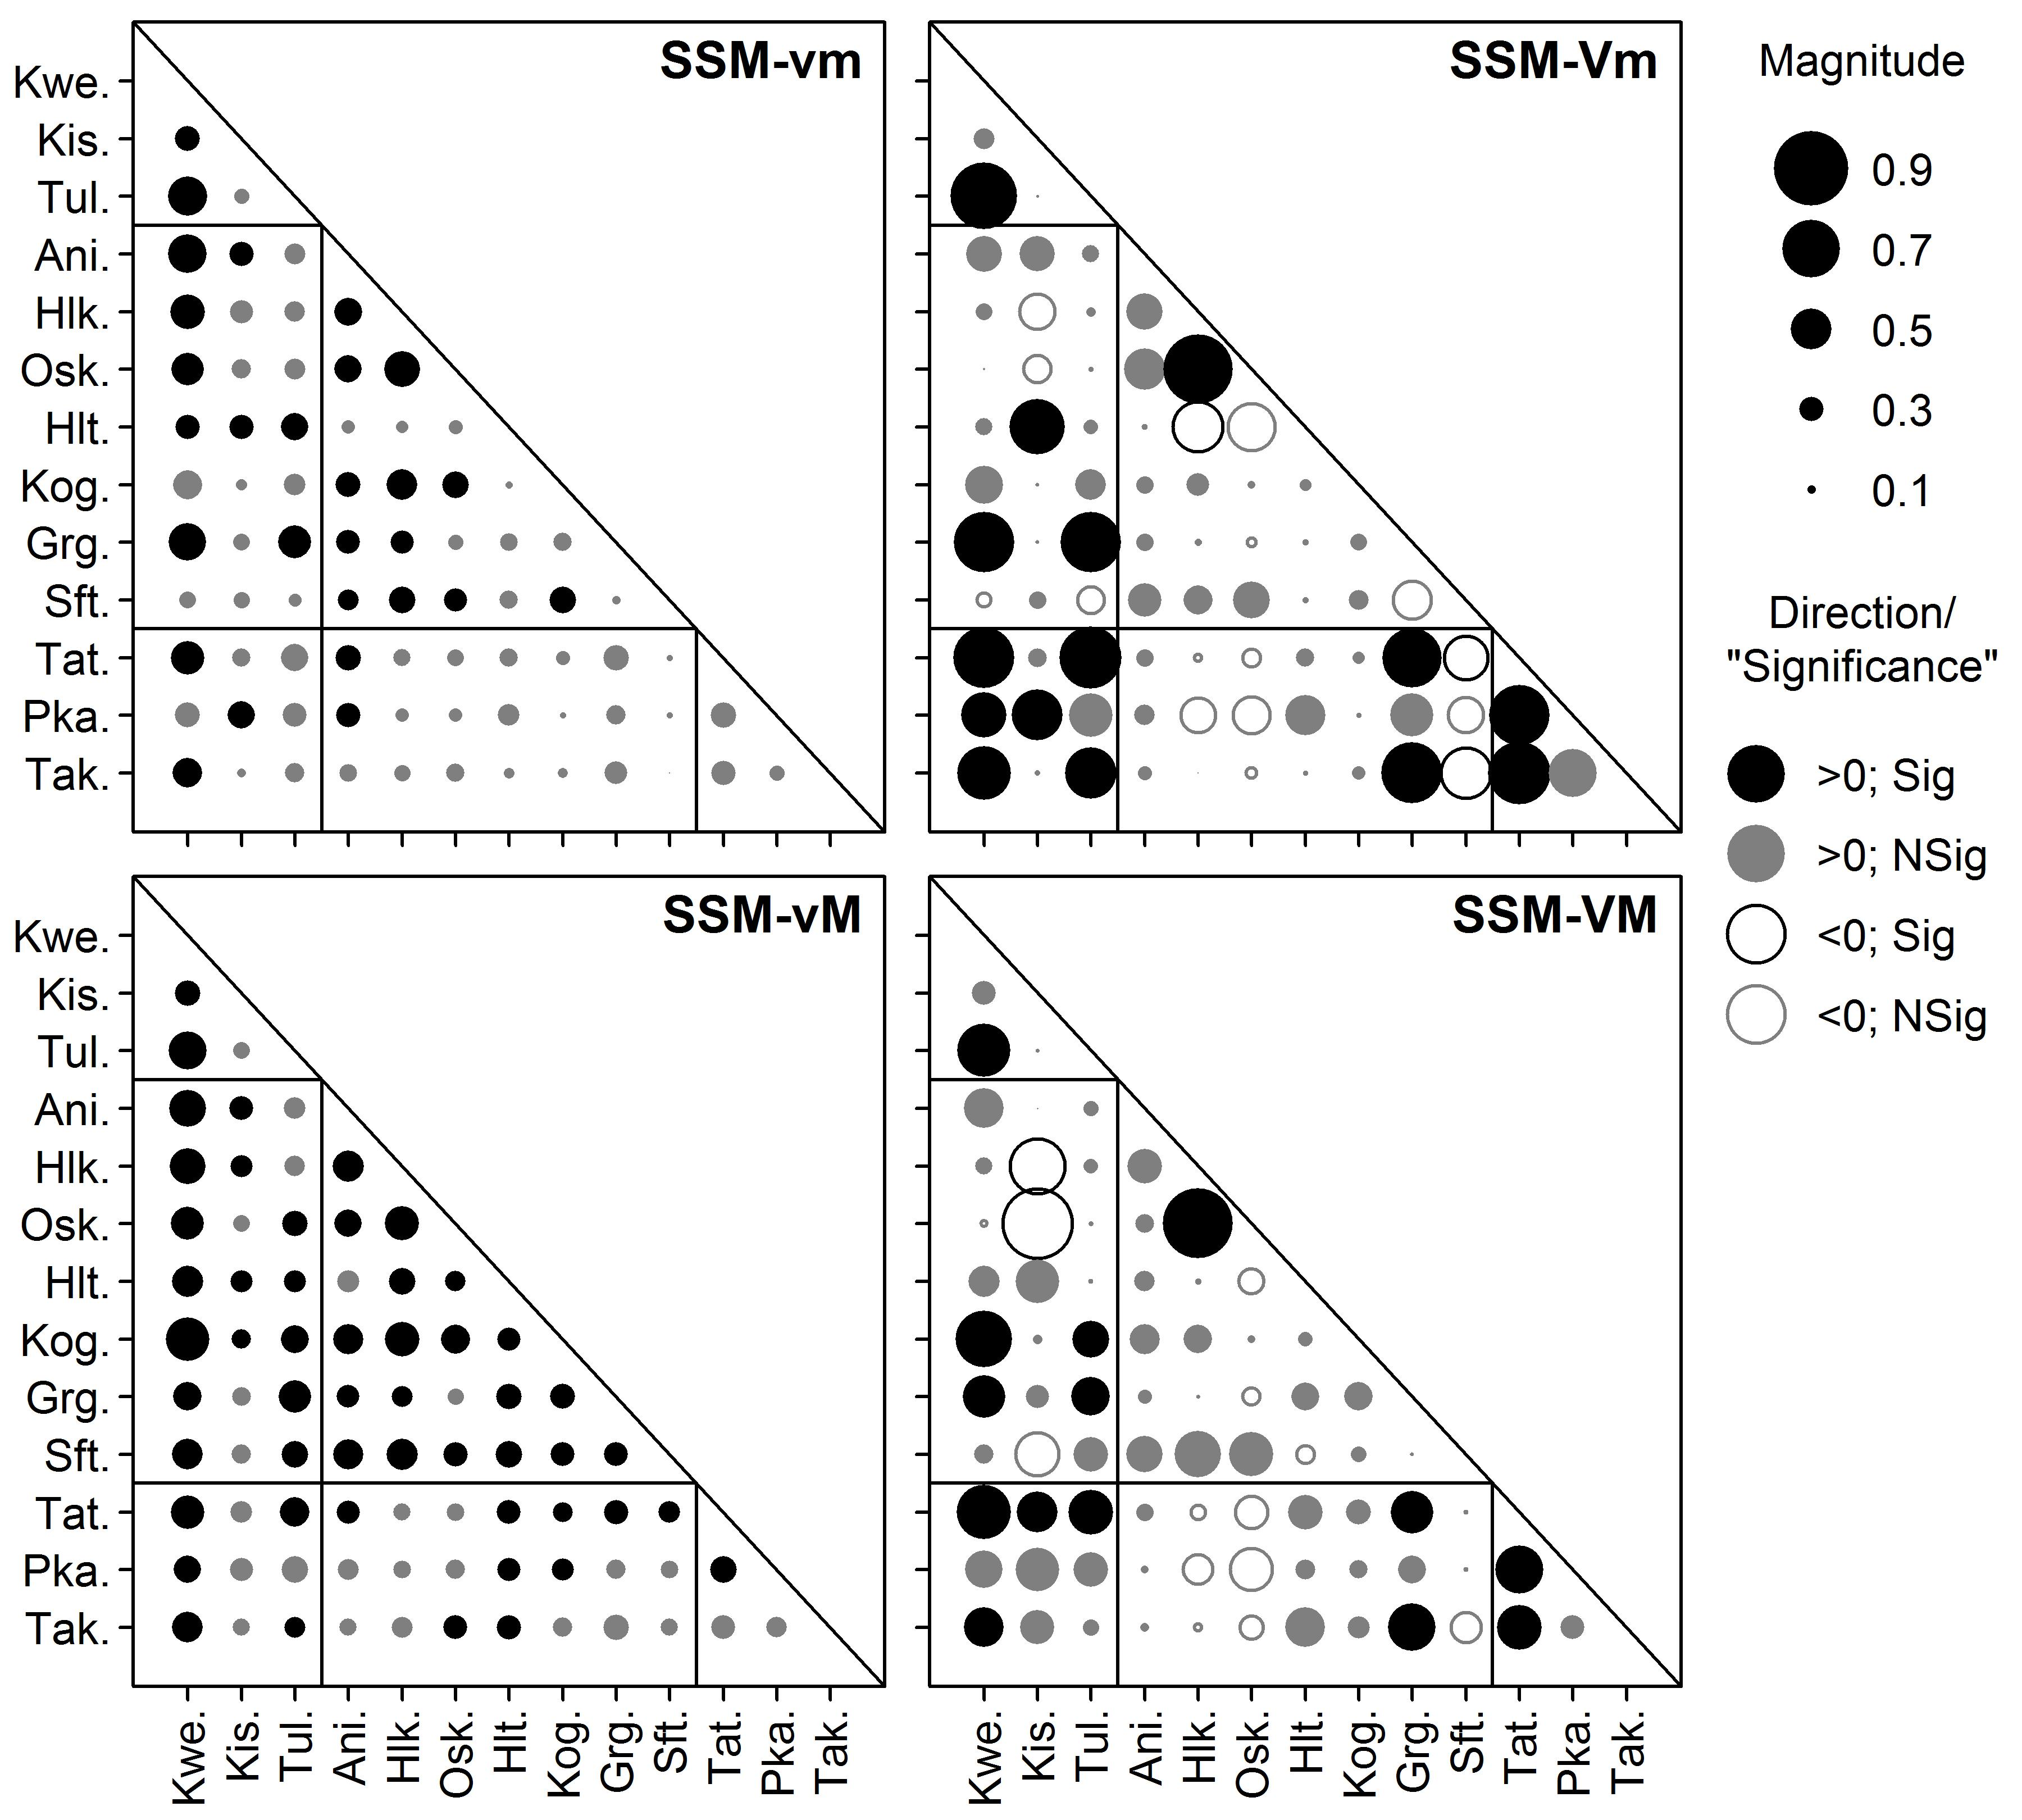
\includegraphics{img/Ch4/rhos.jpg}
  \caption{Caption goes here.}
  \label{fig:rhos}
\end{figure}

\doublespacing

\setlength{\parskip}{6pt plus 2pt minus 1pt}

\bibliography{cites-without-doi.bib,cites-with-doi.bib}


\end{document}
